\documentclass[11pt,reqno]{amsart}

\usepackage[T1]{fontenc}
\usepackage[utf8]{inputenc}
\IfFileExists{lmodern.sty}
 {\usepackage{lmodern}\usepackage{microtype}}
 {\usepackage[expansion=false]{microtype}}% fallback for minimal TeX installs
\usepackage[margin=1.08in]{geometry}
\usepackage{amsmath,amssymb,mathtools}
\usepackage{booktabs,tabularx,array,enumitem,needspace}
\usepackage{tikz}
\usetikzlibrary{arrows.meta,positioning}
\usepackage{xcolor}
    \definecolor{linkblue}{RGB}{24,54,87}
\usepackage[unicode,breaklinks]{hyperref}
    \hypersetup{colorlinks=true,allcolors=linkblue,
    pdftitle={From Exact Counting to Circuit Lower Bounds},
    pdfauthor={moi},
    pdfsubject={Draft 7: a reconstruction of the announced refutation of ETH,
    its circuit consequence, and its verification obligations}}
\urlstyle{same}

\setlength{\emergencystretch}{1.2em}
\setlist{leftmargin=1.6em,itemsep=.18em,topsep=.35em}
\setcounter{tocdepth}{1}

\numberwithin{equation}{section}
\theoremstyle{plain}
\newtheorem{theorem}{Theorem}[section]
\newtheorem{lemma}[theorem]{Lemma}
\newtheorem{proposition}[theorem]{Proposition}
\newtheorem{corollary}[theorem]{Corollary}
\newtheorem{reported}[theorem]{Reported Result}
\theoremstyle{definition}
\newtheorem{definition}[theorem]{Definition}
\newtheorem{hypothesis}[theorem]{Research Hypothesis}
\theoremstyle{remark}
\newtheorem{remark}[theorem]{Remark}

\newcommand{\Z}{\mathbb Z}
\newcommand{\Q}{\mathbb Q}
\newcommand{\F}{\mathbb F}
\newcommand{\poly}{\operatorname{poly}}
\newcommand{\rank}{\operatorname{rank}}
\newcommand{\ind}{\mathbf 1}
\newcommand{\ENP}{\mathrm E^{\mathrm{NP}}}
\newcommand{\NTIME}{\operatorname{NTIME}}
\newcommand{\valtwo}{v_2}
\newcolumntype{Y}{>{\raggedright\arraybackslash}X}
\renewcommand{\thepart}{\Roman{part}}
\newcommand{\parhead}[1]{\par\smallskip\noindent\textit{#1}\enspace\ignorespaces}

%%%%%%%%%%%%%%%%%%%%%%%%%%%%%%%%%%%%%%%%%%%%%%%%%%%%%%%%%%%%%%%%%%%%%%%%%%%%

\title[From exact counting to circuit lower bounds]{From Exact Counting to
Circuit Lower Bounds:\\ A Reconstruction of the Announced Refutation of ETH\\
and Its Verification Obligations}
\author{Jhune Yim}
\address{Independent Researcher}
\email{jhune\_yim@protonmail.com}
\thanks{30 October 2026. An expository reconstruction with explicit
classical inputs and a quantitative synthesis of the reported bounds; no new
refutation of ETH or complete independent audit of that announcement is claimed}
\date{30 October 2026}
\subjclass[2020]{Primary 68Q17; Secondary 68Q06, 68Q25, 68V20, 68T20}
\keywords{Exponential Time Hypothesis, exact counting, circuit lower bounds,
 local reductions, nondeterministic time hierarchy, tensor contraction,
 formal verification, AI-assisted mathematics}

\begin{document}

\begin{abstract}
A manuscript released by OpenAI in October 2026 announces a deterministic,
polynomial-space algorithm for exact counting of fixed-width CNF solutions
in subexponential time. This expository paper reconstructs its reported
circuit consequence, Corollary~1.4, conditional on the stated SAT bounds.
The conclusion is a language in $\ENP$ whose unrestricted fan-in-two
circuit complexity exceeds $cN\sqrt{\log N}$ at infinitely many lengths.
We explain the witness-circuit argument with explicit accounts of lengths,
gates, clauses, oracle access, and quantifiers. An elementary quantitative
transfer theorem distinguishes the circuit scales supported by the sparse,
general-density, and formally specified SAT estimates.
We also prove selected algebraic interfaces of the counter, including
measurement-fiber factorisation, Taylor recovery, low-rank locality,
integral parity truncation, and precision accounting. A variable-overhead
criterion explains both the reach and the limits of substituting the SAT
solver into other algorithms. In particular, a direct encoding gives a
quantitative bound for SNP in its relation-bit parameter; this parameter
must be distinguished from universe size or input length. The estimates do
not by themselves establish subexponential algorithms for all NP problems.
A methodological appendix discusses verification and AI-assisted research.
An accompanying finite-check suite supports the interface calculations;
it does not audit the full announced SAT algorithm or its Lean development.
\end{abstract}

\maketitle
\tableofcontents

%%%%%%%%%%%%%%%%%%%%%%%%%%%%%%%%%%%%%%%%%%%%%%%%%%%%%%%%%%%%%%%%%%%%%%%%%%%%

\section{Introduction}\label{sec:intro}

\subsection{An algorithm that also implies hardness}
The usual story about a faster SAT algorithm concerns problems becoming
easier. One encodes a target problem into SAT, substitutes the new solver,
and obtains a better upper bound. Page~3 of OpenAI's manuscript
\emph{The Exponential Time Hypothesis Is False} \cite{OpenAIPaper} contains
this familiar consequence for counting independent sets, colorings, and
perfect matchings. Immediately afterwards, its Corollary~1.4 goes in the
opposite direction. The sparse SAT speedup implies that a language in
$\ENP$ requires general Boolean circuits of size larger than
$cN\sqrt{\log N}$ at infinitely many input lengths.

That corollary organises this paper. The circuits have fan-in two,
unrestricted fan-out, and no depth bound. The language is computationally
specified, rather than selected by a counting argument, but it need not lie
in NP. The conclusion is not a superpolynomial lower bound and says nothing
directly about $\mathrm P$ versus $\mathrm{NP}$.

The mechanism fits in one paragraph. Choose a unary language whose
nondeterministic exponential running time cannot be halved in the exponent.
A local reduction represents acceptance by an exponentially large 3-CNF
with a small clause decoder. If a small circuit could compute the bits of a
canonical satisfying assignment, a nondeterministic machine could guess that
circuit and build a small circuit asking whether any decoded clause is
violated. Converting that circuit to sparse 3-SAT and running the fast
solver would decide the hard language too quickly. Hence some witness-bit
function requires larger circuits, and the size of the SAT saving determines
how much larger.

\subsection{Contributions}
\begin{enumerate}[label=(\alph*)]
\item A detailed reconstruction of Corollary~1.4 with explicit classical inputs
 (Theorem~\ref{thm:main}), with every length, gate count, clause count, and
 oracle permission recorded. The proof pattern is due to Williams
 \cite{Williams} and the local reduction to Jahanjou, Miles, and Viola
 \cite{JMV}; the quantitative specialisation follows Appendix~C.1 of
 \cite{OpenAIPaper}.
\item An elementary transfer theorem for logarithmic SAT savings
 (Theorem~\ref{thm:general-scale}). It shows that the bound specified for the
 formalization supports only the scale $N\sqrt{\log N}/(\log\log N)^2$
 through this argument (Corollary~\ref{cor:formal-scale}).
\item Short proofs of the algebraic interfaces of the counter
 (Sections~\ref{sec:measurements}--\ref{sec:tensors}), including the
 low-rank matrix construction, the integral parity lift, and a $2$-adic
 precision lemma.
\item A criterion for the variable overhead that an encoding into SAT can
 tolerate (Proposition~\ref{prop:overhead}), and an account of which NP
 problems a refutation of ETH reaches (Section~\ref{sec:np},
 Table~\ref{tab:np-reach}): clause growth is harmless, variable growth by a
 logarithmic factor is not, and lower-bound and upper-bound transfer use
 reductions in opposite directions.
\item A methodological appendix on AI-assisted mathematics with separate
 specification, correctness, resource, and provenance obligations
 (Appendix~\ref{app:ai}). It is a proposal; no implemented system is evaluated.
\end{enumerate}

\subsection{Status of the results used here}\label{sec:status}
We call a result a \emph{Reported Result} when it is asserted in the
manuscript \cite{OpenAIPaper} or specified by its formalisation documentation
\cite{OpenAIScope,OpenAIComparator}, at the version fixed in
Appendix~\ref{app:provenance}. Classical theorems quoted from the literature are identified by their
citations. The interface lemmas and conditional compositions established
here are followed by proofs; a cited classical input is not claimed to
have been proved anew in this paper.
We do not rebuild the Lean development, audit its axioms, or independently
check every construction lemma of the manuscript. The tensor contraction
theorem (Reported Result~\ref{rep:tensor}) and the manuscript's placement,
height, and recursion estimates are external dependencies. We claim no
novelty for sparsification, gate encodings, interpolation, concentration
inequalities, counting-to-sampling reductions, or the witness-circuit method.

Three questions are kept apart throughout: what was publicly released, what
mathematical statements those materials specify, and what has been
independently checked. Evidence for one does not settle the others. A
kernel-checked proof is strong evidence for its formal statement; whether
that statement expresses the intended theorem is a separate question.

\subsection{Related work}\label{sec:related}
ETH and SETH were introduced by Impagliazzo, Paturi, and Zane
\cite{IP,IPZ}; Lokshtanov, Marx, and Saurabh survey their use for
conditional lower bounds \cite{LMS}. Williams \cite{Williams} showed that
algorithms beating exhaustive search for circuit satisfiability imply
circuit lower bounds, and that a refutation of ETH already implies that
$\ENP$ lacks linear-size circuits \cite[Theorem~6.1]{Williams}. Jahanjou,
Miles, and Viola \cite{JMV} supplied local reductions with clause decoders
of near-optimal locality, which make such arguments quantitatively tight.
Chen, Rothblum, Tell, and Yogev \cite{CRTY} show more generally that
disproving certain exponential-time hypotheses requires breakthrough
circuit lower bounds; Corollary~1.4 is a quantitative instance of that
phenomenon.

For comparison, Kannan \cite{Kannan} proved that for every fixed $a$ there
is a language in $\Sigma_2\mathrm P\cap\Pi_2\mathrm P$ without
$O(N^a)$-size circuits, and showed that $\Sigma_3\mathrm E\cap\Pi_3\mathrm E$
contains languages of maximum circuit complexity. Miltersen, Vinodchandran,
and Watanabe \cite{MVW} lowered the class to
$\Delta_3\mathrm E=\mathrm E^{\Sigma_2\mathrm P}$ by binary search, which
remained the smallest class known to require exponential circuit
complexity until Chen, Hirahara, and Ren \cite{CHR} proved near-maximum
lower bounds for $\Sigma_2\mathrm E$ and for symmetric exponential time
with one bit of advice; Li \cite{LiZ} removed the advice and obtained an
almost-everywhere bound for symmetric exponential time. All of these
classes contain $\ENP$, so these results do not give lower bounds for
$\ENP$. Section~\ref{sec:main-proof} explains why generic hard-table search
stops at $\Delta_3\mathrm E$.

In the literature preceding the announcement, superlinear lower bounds for
$\ENP$ over general fan-in-two circuits were open. Williams notes that, to
the best of his knowledge, it was not known that $\ENP$ lacks linear-size
circuits \cite[Section~1.1.1, footnote~5]{Williams}, and Find, Golovnev,
Hirsch, and Kulikov state that superlinear bounds are unknown even for
functions in $\ENP$ \cite[Section~1.1]{FGHK}. For polynomial-time computable
functions over the full binary basis, the $3.1N-o(N)$ lower bound of Li and
Yang is a relevant benchmark \cite{LiYang}. The issue addressed by the
announced corollary is a superlinear bound for a language in $\ENP$.

Against this background, the qualitative consequence is already notable:
Williams proved that if ETH is false, then $\ENP$ does not have
linear-size circuits \cite[Theorem~6.1]{Williams}, that is,
\[
 \neg\mathrm{ETH}\ \Longrightarrow\ \ENP\not\subseteq\mathrm{SIZE}(O(N)).
\]
A correct refutation of ETH would therefore settle this open question
without further assumptions. Corollary~1.4 adds an explicit growing factor,
$\sqrt{\log N}$ at infinitely many lengths, and Section~\ref{sec:scale}
shows how that factor depends on which SAT bound is used.

The counting side builds on counting sparsification \cite{DHM} and the
counting-to-sampling principle \cite{JVV}. A separate record released by
Anthropic on 27 October 2026 \cite{Anthropic} announces an independent
deterministic $2^{o(n)}$ algorithm for 3-SAT that also counts satisfying
assignments; it is not analyzed here.

\subsection{Organisation and conventions}
Part~\ref{part:eth} develops ETH and the direction of reductions.
Part~\ref{part:consequences} states the reported bounds and derives their
consequences, with Corollary~1.4 at the center. Part~\ref{part:mechanism}
explains the algebra of the counter and the formal statement it is checked
against. Appendix~\ref{app:ai} turns the same obligations into a proposal for
research systems, separately from the mathematical exposition.

Logarithms are to base two unless written $\ln$. Iterated logarithms are used
only for sufficiently large arguments; bounded sizes are handled directly. A
CNF has $n$ \emph{declared} variables and $m$ clauses. Unused variables
remain declared, and $\#F$ counts assignments to all of them. Time and space
bounds refer to bit operations and stored bits unless stated otherwise.
Constants written $O_k$ may depend on the fixed width $k$, never on a width
that grows with the input. We reserve $k$ for clause width and $\ell$ for a
solution-size parameter.

%%%%%%%%%%%%%%%%%%%%%%%%%%%%%%%%%%%%%%%%%%%%%%%%%%%%%%%%%%%%%%%%%%%%%%%%%%%%

\part{ETH and the direction of reductions}\label{part:eth}

\section{Satisfiability, ETH, and SETH}\label{sec:eth}

A literal is a Boolean variable or its negation, and a $k$-CNF is a
conjunction of clauses with at most $k$ literals each. The formula
\[
 (x_1\lor\neg x_2\lor x_3)\land(x_2\lor x_4\lor\neg x_5)
\]
requires a true literal in each clause. Exhaustive search decides $k$-SAT in
$2^n\poly(n+m)$ time for fixed $k$. That bound comes from the size of the
search space; it is not a proof that assignments must be inspected one at a
time. ETH asks whether some aggregation can remove a positive linear rate
from the exponent in the worst case.

An algorithm is \emph{subexponential in the variable count} if it runs in
time $2^{h(n)}\poly(n+m)$ with $h(n)=o(n)$. Both $2^{\sqrt n}$ and
$2^{n/\log n}$ qualify; $1.01^n$ does not. Such a bound can still be
superpolynomial: at $n=10\,000$, the first example has exponent $100$ in
place of $10\,000$, and $2^{100}$ is not a practical budget.

Decision, search, and exact counting are different tasks. Counting implies
decision through a positivity test. The converse does not hold in general:
2-SAT is decidable in polynomial time, whereas exact \#2-SAT is
$\#\mathrm P$-complete. Declared variables matter for counting. The formula
$x_1$ on $n$ declared variables has $2^{n-1}$ satisfying assignments, the
empty conjunction has $2^n$, and a formula with an empty clause has none.

For fixed $k\ge3$ put
\begin{equation}\label{eq:sk}
 s_k=\inf\{\delta\ge0:\text{$k$-SAT has a deterministic algorithm in time }
                 2^{\delta n}(n+m)^{O(1)}\}.
\end{equation}
The polynomial degree may depend on the algorithm and on $k$. Normalisation
leaves at most $O_k(n^k)$ distinct nonempty clauses, so the input length is
polynomial in $n$.

\begin{definition}[ETH and SETH \cite{IP,IPZ}]
ETH is the assertion $s_3>0$. SETH is the assertion $\lim_{k\to\infty}s_k=1$;
the sequence $s_k$ is nondecreasing and bounded by one.
\end{definition}
Spelled out, SETH says that for every fixed $\varepsilon\in(0,1)$ some fixed
width $k$ admits no deterministic $2^{(1-\varepsilon)n}\poly(n+m)$
algorithm. The width is chosen after $\varepsilon$ and then held fixed as $n$
grows.

\begin{proposition}\label{prop:refute}
A deterministic $2^{o(n)}\poly(n+m)$ algorithm for 3-SAT gives $s_3=0$. Such
an algorithm for every fixed width gives $s_k=0$ for all $k\ge3$,
contradicting ETH and SETH.
\end{proposition}
\begin{proof}
For fixed $\delta>0$, eventually $h(n)\le\delta n$. Finitely many smaller
lengths are absorbed into a constant, so every positive $\delta$ is
admissible in \eqref{eq:sk}.
\end{proof}

ETH is a worst-case statement in one parameter. It does not assert that
typical or random instances are hard, nor that every NP-complete problem
needs a linear exponent in every natural size measure. If
$\mathrm P=\mathrm{NP}$ then ETH fails; a subexponential upper bound proves
neither side of $\mathrm P$ versus $\mathrm{NP}$.

\section{Sizes, sparsification, and reductions}\label{sec:reductions}
A reduction $A\le_p B$ turns instances of $A$ into instances of $B$, so an
algorithm for $B$ solves $A$. To use a SAT algorithm for a target problem,
one needs an encoding of the target \emph{into} SAT with controlled variable
count. Lower bounds travel in the other direction.

Sizes matter in both directions. A linear-size reduction from 3-SAT to
3-coloring produces $O(n+m)$ vertices, and $m$ can be of order $n^3$. A
$2^{o(v)}$ coloring algorithm therefore does not immediately give $2^{o(n)}$
for SAT. Sparsification removes this mismatch.

\begin{theorem}[Sparsification \cite{IPZ}; counting version \cite{DHM}]
\label{thm:sparsification}
For fixed $k$ and fixed $\eta>0$ there is $C_{k,\eta}$ such that every
$n$-variable $k$-CNF is a disjunction of at most $2^{\eta n}$ formulas on the
same declared variables, each with at most $C_{k,\eta}n$ clauses, computable
in $2^{\eta n}\poly(n+m)$ time. In the counting version the branches have
disjoint sets of satisfying assignments, so $\#F=\sum_i\#F_i$.
\end{theorem}
Equisatisfiability alone would not justify the sum; an assignment shared by
two branches would be counted twice.

\begin{proposition}[Lower-bound transfer]\label{prop:lower-transfer}
Fix $a>0$. Suppose that for every fixed $C$, 3-SAT instances with $m\le Cn$
reduce in polynomial time to instances of a problem $X$ with size parameter
$N=O_C(n^a)$ and polynomial bit length. If $X$ has a
$2^{o(N^{1/a})}\poly(|I|)$ algorithm, then $s_3=0$.
\end{proposition}
\begin{proof}
Given $\delta>0$, sparsify with $\eta=\delta/2$. Every branch has density
$C_{3,\eta}$, independent of $n$, and is solved in $2^{o(n)}\poly(n+m)$
time. The total is eventually at most $2^{\delta n}\poly(n+m)$.
\end{proof}
The proof produces arbitrarily small constant rates, as \eqref{eq:sk}
requires; $2^{\eta n}$ is not called subexponential for fixed $\eta$. For a
planarisation with $N=O(n^2)$ this explains the ETH-based exclusion of
$2^{o(\sqrt N)}$ planar algorithms. It gives no encoding of arbitrary planar
instances into $O(\sqrt N)$ SAT variables. Similarly, the failure of an
ETH-based exclusion of $f(\ell)N^{o(\ell)}$ time for parameterised Clique
\cite{Chen,LMS} does not by itself construct such an algorithm.

%%%%%%%%%%%%%%%%%%%%%%%%%%%%%%%%%%%%%%%%%%%%%%%%%%%%%%%%%%%%%%%%%%%%%%%%%%%%

\part{The reported counter and its consequences}\label{part:consequences}

\section{The reported bounds}\label{sec:reported}

OpenAI's announcement of 26 October 2026 reports a natural-language proof
obtained on 16 October and a Lean formalisation on 17 October
\cite{OpenAIAnnouncement}. We analyse the 25 October revision of the
manuscript.

\begin{reported}[{\cite[Theorem~1.1]{OpenAIPaper}}]\label{rep:counter}
For every fixed $k\ge2$ there is a deterministic algorithm that computes
$\#F$ for a $k$-CNF with $n\ge20$ declared variables and $m$ clauses in time
\begin{equation}\label{eq:general-time}
 (n+m)^{O_k(1)}\,2^{O_k(n\log\log n/\sqrt{\log n})}
\end{equation}
and $(n+m)^{O_k(1)}$ bits of space. For every fixed $D>0$, inputs with
$m\le Dn$ admit the sharper time bound
\begin{equation}\label{eq:density-time}
 (n+m)^{O_{k,D}(1)}\,2^{O_{k,D}(n/\sqrt{\log n})}.
\end{equation}
\end{reported}

\begin{reported}[{\cite{OpenAIScope,OpenAIComparator}}]\label{rep:scope}
For each fixed $k$, the formalisation specifies one fixed deterministic
machine that exactly counts satisfying assignments of $k$-CNF formulas given
by canonical encodings of bit length $L$, in time
\begin{equation}\label{eq:scope-time}
 (L+1)^{O_k(1)}\,2^{O_k(\rho(n))},\qquad
 \rho(n)=\frac{n(\log\log n)^2}{\sqrt{\log n}},
\end{equation}
with polynomially bounded visited space at every prefix of the execution.
\end{reported}

The output has at most $n+1$ bits, and small $n$ is handled by enumeration.
The manuscript proves \eqref{eq:general-time} and \eqref{eq:density-time} in
its Appendix~D; the scope document does not identify them as the bound of the
comparator theorem. Table~\ref{tab:bounds} keeps the three statements
apart. Each exponent is $o(n)$, because every fixed power of $\log\log n$ is
$o(\sqrt{\log n})$.

\begin{table}[htbp]
\caption{Three quantitative statements in the public materials.}
\label{tab:bounds}
\small
\begin{tabularx}{\textwidth}{@{}lYl@{}}
\toprule
Source & Exponent of the time bound & Inputs\\
\midrule
Manuscript, Theorem 1.1 & $O_k(n\log\log n/\sqrt{\log n})$ & all densities\\
Manuscript, fixed density & $O_{k,D}(n/\sqrt{\log n})$ & $m\le Dn$\\
Formalisation scope & $O_k(n(\log\log n)^2/\sqrt{\log n})$ & all densities\\
\bottomrule
\end{tabularx}
\end{table}

\begin{corollary}\label{cor:hypotheses}
If Reported Result~\ref{rep:counter} or \ref{rep:scope} holds, then ETH, SETH,
counting ETH, and Gap-ETH fail, as do their bounded-error randomised versions.
\end{corollary}
\begin{proof}
Test positivity of the count and apply Proposition~\ref{prop:refute}.
Counting ETH excludes a $2^{o(n)}$ algorithm for exactly this counting task
\cite{DHM}. Gap-ETH concerns distinguishing satisfiable 3-CNFs from those in
which every assignment violates a fixed fraction of clauses; exact decision
solves that promise problem. A deterministic algorithm is in particular a
bounded-error randomised one.
\end{proof}

\section{Count-preserving encodings}\label{sec:encodings}

\subsection{Clause polynomials}
Write a positive literal as $x_i$ and a negative one as $1-x_i$, and put
\begin{equation}\label{eq:clause-polynomial}
 \Phi_e(x)=1-\prod_{\lambda\in e}\bigl(1-\lambda(x)\bigr),\qquad
 \#F=\sum_{x\in\{0,1\}^n}\prod_e\Phi_e(x).
\end{equation}
For example, $(x_1\lor\neg x_2)\land(x_2\lor x_3)$ has count
$\sum_x[1-(1-x_1)x_2][1-(1-x_2)(1-x_3)]=4$. The identity is still an
exponential sum; the counter's task is to control its coupling.

\subsection{Unique extensions}
An encoding of $F(x)$ as $G(x,z)$ has \emph{unique extensions} if every
satisfying assignment of $F$ extends to exactly one satisfying assignment of
$G$ and every other assignment extends to none. Then $\#G=\#F$.

\begin{lemma}[Gate and circuit encodings]\label{lem:gates}
The clauses $(\neg u\lor z)\land(\neg v\lor z)\land(u\lor v\lor\neg z)$ force
$z=u\lor v$. More generally, a fan-in-two circuit with $q$ inputs and $t$
noninput gates has a 3-CNF encoding with $q+t$ declared variables and at most
$4t+1$ clauses that is satisfiable exactly when the circuit accepts some
input; gate variables extend each accepted input uniquely. For $q\ge1$ the
clause count is at most $5(q+t)$.
\end{lemma}
\begin{proof}
For the OR gate: if $u=v=0$ the third clause forces $z=0$, and otherwise one
of the first two forces $z=1$. For an arbitrary two-input gate $g$, forbid
each of the four triples $(u,v,z)$ with $z\ne g(u,v)$ by one clause of width
at most three. Unary and constant gates need fewer clauses. Topological
evaluation determines every gate variable from the inputs, and a unit clause
on the output selects accepted inputs. The counts follow.
\end{proof}

\begin{lemma}[Occurrence splitting]\label{lem:cycle}
Replace the $s\ge2$ occurrences of a variable by copies $x_1,\dots,x_s$ with
their signs, and add $(\neg x_1\lor x_2)\land\dots\land(\neg x_{s-1}\lor
x_s)\land(\neg x_s\lor x_1)$. All copies agree, counts are preserved, and
each copy lies in at most three clauses.
\end{lemma}
\begin{proof}
If one copy is true, implication around the cycle makes all copies true;
otherwise all are false. Each copy occurs in its original clause and in two
cycle clauses.
\end{proof}
Splitting bounds occurrences but increases the number of variables, and that
increase must be charged to the running time (Section~\ref{sec:upper}).

\subsection{Counting gives search and exact sampling}
\begin{proposition}[Self-reduction \cite{JVV}]\label{prop:sampling}
A deterministic exact counter for fixed-width CNF yields a deterministic
search algorithm with at most $n+1$ counter calls, and an exact uniform
sampler with the same number of calls and $O(n^2)$ expected random bits.
\end{proposition}
\begin{proof}
Under a prefix, let $Z$ be the number of extensions and $Z_0,Z_1$ the numbers
after fixing the next variable; $Z=Z_0+Z_1$, so one new call per level
suffices. Fixing a variable removes satisfied clauses and false literals, so
the width does not grow, and the remaining declared variables are kept. For
search, follow a bit with positive conditional count. For sampling, choose
$b$ with probability $Z_b/Z$. For each satisfying assignment the product of
conditional probabilities telescopes to $1/\#F$. Draw $\lceil\log Z\rceil$
random bits and reject values $\ge Z$; acceptance has probability at least
one half and $\log Z\le n$. An initial count of zero is reported as failure.
\end{proof}

\section{A reconstruction of Corollary 1.4}\label{sec:main-proof}

\subsection{Statement}
\begin{definition}[Circuits and $\ENP$]\label{def:circuits}
For a language $L$, $C_L(N)$ is the minimum number of noninput gates of a
circuit computing $L$ on $\{0,1\}^N$. Gates compute arbitrary Boolean
functions of at most two inputs, fan-out is unrestricted, and no uniformity
is imposed. Put $\ENP=\bigcup_{c>0}\operatorname{DTIME}(2^{cN})^{\mathrm{NP}}$,
with oracle queries charged to the time budget, so queries may have length
$2^{O(N)}$.
\end{definition}

\begin{reported}[{\cite[Corollary~1.4]{OpenAIPaper}}]\label{rep:circuits}
There are $L\in\ENP$ and $c>0$ with $C_L(N)>cN\sqrt{\log N}$ for infinitely
many $N$.
\end{reported}

The quantifiers are
\begin{equation}\label{eq:io}
 \exists L\in\ENP\ \exists c>0\ \forall N_0\ \exists N\ge N_0:\quad
 C_L(N)>cN\sqrt{\log N}.
\end{equation}
This rules out linear-size circuits for $L$, since $\sqrt{\log N}\to\infty$
along the hard lengths. It is not an almost-everywhere bound and does not
exclude $C_L(N)=O(N\sqrt{\log N})$.

\parhead{What generic hard-table search does and does not show.}
By counting, almost every Boolean function on $N$ inputs requires
$\Omega(2^N/N)$ gates. Selecting a hard table within a specified uniform
class is a further task. Given a prefix $p$, the completion question has
the form
\[
 \exists F\succeq p\quad\forall C\text{ of size at most }s:
                         \quad F\ne\operatorname{tt}(C),
\]
where $F$ has $2^N$ bits and $\operatorname{tt}(C)$ is the full truth table
of $C$. For $s\le2^N$, comparing these explicit tables takes time
polynomial in their exponential description length. Thus this is a
$\Sigma_2^{\mathrm P}$ completion query on exponentially long data.
Adaptive prefix search uses exponentially many such queries, giving the
generic upper bound $\mathrm E^{\Sigma_2\mathrm P}=\Delta_3\mathrm E$;
it does not establish an $\ENP$ construction, or a
$\Sigma_2\mathrm E$ construction by that reasoning alone.

This is not a proof that an NP oracle cannot solve the completion problem,
nor a separation of these uniform classes. Constructions in smaller classes
require additional ideas. Kannan claimed that
$\Sigma_2\mathrm E\cap\Pi_2\mathrm E$ requires exponential circuit size;
Miltersen, Vinodchandran, and Watanabe pointed out a gap in the proof
\cite{MVW}, and Chen, Hirahara, and Ren establish the claim up to one bit
of advice \cite[Section~1]{CHR}.

Avoiding the oracle altogether by enumerating circuits does not help at
the scale of Corollary~1.4. There are $2^{\Theta(s\log(s+N))}$ syntactically
distinct fan-in-two circuits with $s\ge N$ gates on $N$ inputs. This number
exceeds every bound $2^{O(N)}$ as soon as $s\log s=\omega(N)$, and in
particular at $s=N\sqrt{\log N}$. This is a limitation of that enumeration,
not a lower bound on every possible construction. The witness-circuit argument
instead guesses one circuit nondeterministically and uses its structure
for a fast, exact validation inside a time-hierarchy contradiction.

\subsection{The SAT premise and the machine model}
Only the positivity of counts is used below.
\begin{definition}[Sparse SAT assumption $\mathcal A_g$]\label{def:assumption}
Let $g$ be an eventually positive function. $\mathcal A_g$ asserts that there
are constants $A,b>0$ and a deterministic oracle-free multitape Turing machine
that decides every 3-CNF with $V$ declared variables and at most $5V$
clauses in time $V^b2^{AV/g(V)}$ for all sufficiently large $V$.
\end{definition}

\begin{lemma}[Model conversion]\label{lem:model}
Suppose an algorithm on a random-access machine runs in time $T(V)$ and its
memory contents, including addresses, occupy at most $S(V)=V^{O(1)}$ bits.
Then a multitape Turing machine simulates it in time $T(V)\cdot V^{O(1)}$.
In particular, Reported Result~\ref{rep:counter} with $k=3$ and $D=5$ gives
$\mathcal A_{a_0}$ for $a_0(V)=\sqrt{\log V}$.
\end{lemma}
\begin{proof}
Store memory as a list of address--value pairs on one tape, of length
$O(S)$. Each random-access step is simulated by a constant number of scans
of this tape and of a polynomial-length work tape, at cost $S^{O(1)}$.
The multiplicative overhead is absorbed into $V^b$. For the second claim,
a 3-CNF with at most $5V$ clauses has fixed density, and positivity of the
count decides satisfiability.
\end{proof}
If the comparator's fixed machine is already a multitape Turing machine, the
lemma is not needed for Reported Result~\ref{rep:scope}.

\subsection{A hard unary language and a local decoder}
The following are established results, not consequences of the announced
algorithm.

\begin{theorem}[Unary nondeterministic hierarchy \cite{Zak,Williams}]
\label{thm:hierarchy}
For time-constructible bounds with $t_1(n+1)=o(t_2(n))$ there is a unary
language in $\NTIME(t_2)\setminus\NTIME(t_1)$ on multitape Turing machines.
Fix
\begin{equation}\label{eq:hard-unary}
 H\subseteq\{1\}^*,\qquad H\in\NTIME(2^n)\setminus\NTIME(2^{n/2}).
\end{equation}
\end{theorem}
The unary form lets a canonical witness be indexed by the input length alone.

Apply the local reduction of Jahanjou, Miles, and Viola
\cite[Theorem~1 and Section~6]{JMV} to a fixed machine for $H$ on input
$1^n$, with time bound $T=2^nn^{O(1)}$. With a fixed locality parameter it
produces a decoder $D_n$ for a 3-CNF $\Phi_n$ such that:
\begin{enumerate}[label=(\roman*)]
\item clause addresses have $q(n)=n+O(\log n)$ bits;
\item variable labels have at most $dn$ bits for a fixed integer $d$; we pad
 them to exactly $N=dn$ bits and declare all $2^{dn}$ variables;
\item $D_n$ outputs three labels and three signs, and each output bit
 depends on at most a fixed number $w$ of address bits;
\item $D_n$ is evaluable in time polynomial in $n$, and $\Phi_n$ is
 satisfiable exactly when $1^n\in H$.
\end{enumerate}
Repeated clauses and padded unused variables do not affect satisfiability.
Locality is what keeps the decoder circuit linear in $n$:

\begin{lemma}[Recovering constant supports]\label{lem:support}
Let $f\colon\{0,1\}^q\to\{0,1\}$ depend on at most $w$ coordinates, $w$
fixed, and be evaluable in polynomial time. Its set of relevant coordinates
and its truth table on them can be computed in polynomial time from the
values of $f$ on inputs of Hamming weight at most $w$. Consequently $D_n$ has
a uniformly constructible fan-in-two circuit with $O(n)$ gates.
\end{lemma}
\begin{proof}
Let $S$ be the set of relevant coordinates. If $i\in S$, some pair of
inputs differing only in coordinate $i$ has different values. Zeroing every
coordinate outside $S$ in both inputs preserves the values, and both new
inputs are supported in $S$, hence have weight at most $w$. Irrelevant
coordinates never produce a difference. Comparing all such neighboring pairs
among the $O(q^w)$ low-weight inputs therefore recovers $S$, and evaluations
supported in $S$ give the truth table. A function of at most $w$ bits has a
circuit of constant size, and $D_n$ has $O(n)$ output bits.
\end{proof}

\subsection{A canonical witness language}
For satisfiable $\Phi_n$, let $\alpha_n\in\{0,1\}^{2^{dn}}$ be its
lexicographically first satisfying assignment, with variables ordered by
label. Define
\begin{equation}\label{eq:witness-language}
 W(i)=\begin{cases}
 \alpha_n[i],& |i|=dn \text{ and } \Phi_n \text{ is satisfiable},\\
 0,&\text{otherwise}.
 \end{cases}
\end{equation}
The input $i$ addresses one bit of an exponentially long assignment; a
circuit for $W$ at length $dn$ represents the whole assignment through its
truth table.

\begin{lemma}\label{lem:witness-class}
$W\in\ENP$.
\end{lemma}
\begin{proof}
On input length $N=dn$, construct $D_n$ and write all $2^{q(n)}$ clauses,
of total length $2^{O(n)}$. One NP query decides satisfiability. If the
formula is satisfiable, recover $\alpha_n$ bit by bit, asking whether the
current prefix followed by $0$ has a satisfying extension. This uses
$2^{dn}$ queries of length $2^{O(n)}$ and $2^{O(N)}$ time in total.
\end{proof}
The exponential oracle queries are used only here. The fast algorithm for $H$
below uses no oracle.

\subsection{The guessed circuit and its violation test}
Suppose a circuit $C$ with at most $s_n$ gates computes $W$ on inputs of
length $dn$. It defines the assignment $i\mapsto C(i)$ to all variables of
$\Phi_n$, and it has a description of $O(s_n\log(s_n+n))$ bits. For an
address $z$, let $D_n(z)$ give labels $\lambda_j(z)$ and negation bits
$\sigma_j(z)$ for $j=1,2,3$. The value of the $j$-th literal is
$C(\lambda_j(z))\oplus\sigma_j(z)$. Define
\begin{equation}\label{eq:violation}
 B_C(z)=\bigwedge_{j=1}^3\neg\bigl(C(\lambda_j(z))\oplus\sigma_j(z)\bigr).
\end{equation}
It uses three copies of $C$, the decoder, and $O(1)$ further gates, so it
has $q(n)$ inputs and at most $3s_n+O(n)$ gates.

\begin{lemma}\label{lem:violation}
The assignment defined by $C$ satisfies $\Phi_n$ if and only if $B_C$ is
unsatisfiable. If $\Phi_n$ is unsatisfiable, then $B_C$ is satisfiable for
every circuit $C$.
\end{lemma}
\begin{proof}
$B_C(z)=1$ exactly when all three literals of clause $z$ are false. If
$\Phi_n$ is unsatisfiable, the assignment defined by $C$ violates some
clause.
\end{proof}

Lemma~\ref{lem:gates} encodes $B_C$ as a 3-CNF. Padding with unused
variables gives, for a fixed constant $B$, a formula with
\begin{equation}\label{eq:U}
 U_n=3s_n+Bn
\end{equation}
variables and at most $5U_n$ clauses. This small formula, not $\Phi_n$, is
what the solver receives. Table~\ref{tab:sizes} lists the lengths involved.

\begin{table}[htbp]
\caption{Sizes in the circuit argument.}
\label{tab:sizes}
\small
\begin{tabularx}{\textwidth}{@{}lYl@{}}
\toprule
Symbol & Meaning & Scale\\
\midrule
$n$ & length of the unary input & time parameter\\
$q(n)$ & address of one clause of $\Phi_n$ & $n+O(\log n)$\\
$N=dn$ & address of one assignment bit & linear in $n$\\
$2^N$ & declared variables of $\Phi_n$ & exponential in $n$\\
$s_n$ & gates of the guessed circuit & about $\eta n\sqrt{\log n}$\\
$U_n$ & variables of the encoded violation test & $3s_n+Bn$\\
\bottomrule
\end{tabularx}
\end{table}

\subsection{The exponent calculation}
Assume $\mathcal A_{a_0}$ with constant $A$. Fix a rational
$0<\eta<1/(12A)$ and put
\begin{equation}\label{eq:threshold}
 s_n=\bigl\lfloor\eta n\lfloor\sqrt{\lfloor\log n\rfloor}\rfloor\bigr\rfloor,
\end{equation}
which is computable in time polynomial in $n$ and asymptotic to
$\eta n\sqrt{\log n}$. Then
\[
 U_n=(3\eta+o(1))\,n\sqrt{\log n},\qquad \log U_n=\log n+O(\log\log n),
 \qquad \sqrt{\log U_n}\sim\sqrt{\log n},
\]
and therefore
\begin{equation}\label{eq:critical-exponent}
 U_n^b\,2^{AU_n/\sqrt{\log U_n}}=2^{(3A\eta+o(1))n}.
\end{equation}
Since $3A\eta<1/4$, this is eventually below $2^{n/4}$. Guessing $C$,
constructing $D_n$, and writing the encoding take time polynomial in $n$,
because $s_n=n(\log n)^{O(1)}$.

\begin{theorem}[Reconstruction of Corollary~1.4]\label{thm:main}
Assumption $\mathcal A_{a_0}$, together with Theorem~\ref{thm:hierarchy} and
the local reduction of \cite{JMV}, implies the conclusion of Reported
Result~\ref{rep:circuits}, with $L=W$.
\end{theorem}
\begin{proof}
Suppose $C_W(dn)\le s_n$ for all sufficiently large $n$. On input $1^n$, a
nondeterministic machine guesses a well-formed circuit with at most $s_n$
gates and $dn$ inputs, builds $B_C$ and its sparse encoding, runs the
deterministic solver, and accepts exactly when the solver reports
unsatisfiability. Nonunary inputs are rejected.

If $1^n\in H$, the circuit computing $W$ at length $dn$ computes
$\alpha_n$, and by Lemma~\ref{lem:violation} that branch accepts. If
$1^n\notin H$, Lemma~\ref{lem:violation} makes every branch reject. By
\eqref{eq:critical-exponent}, the machine runs in time at most $2^{n/2}$ for
large $n$; finitely many small inputs are hardwired. This places $H$ in
$\NTIME(2^{n/2})$, contradicting \eqref{eq:hard-unary}.

Hence $C_W(dn)>s_n$ for infinitely many $n$. With $N=dn$ and
$\sqrt{\log(dn)}\sim\sqrt{\log n}$, the bound $C_W(N)>cN\sqrt{\log N}$ holds
on that sequence for $c=\eta/(2d)$ and large $N$. Lemma~\ref{lem:witness-class}
gives $W\in\ENP$.
\end{proof}

\begin{figure}[htbp]
\centering
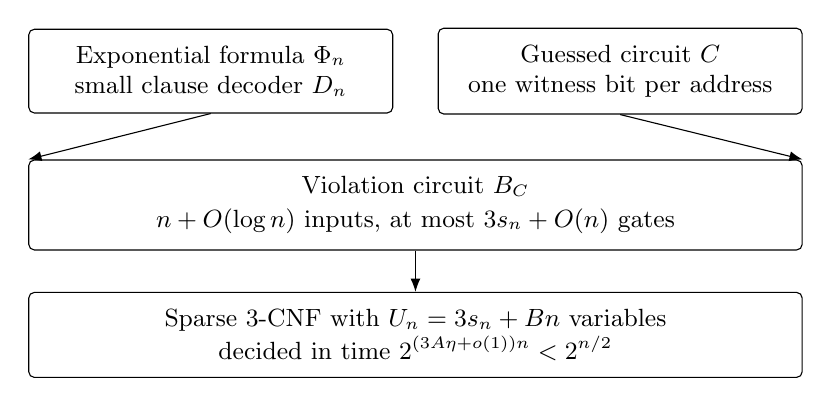
\begin{tikzpicture}[>=Latex,
 box/.style={draw,rounded corners=2pt,align=center,inner sep=6pt,
 font=\small,text width=42mm}]
\node[box] (formula) at (-2.6,0)
 {Exponential formula $\Phi_n$\\small clause decoder $D_n$};
\node[box] (witness) at (2.6,0)
 {Guessed circuit $C$\\one witness bit per address};
\node[box,text width=94mm] (test) at (0,-1.7)
 {Violation circuit $B_C$\\[1pt]
 \mbox{$n+O(\log n)$ inputs, at most $3s_n+O(n)$ gates}};
\node[box,text width=94mm] (sat) at (0,-3.35)
 {\mbox{Sparse 3-CNF with $U_n=3s_n+Bn$ variables}\\[1pt]
 \mbox{decided in time $2^{(3A\eta+o(1))n}<2^{n/2}$}};
\draw[->] (formula.south)--(test.north west);
\draw[->] (witness.south)--(test.north east);
\draw[->] (test)--(sat);
\end{tikzpicture}
\caption{The compression behind the hierarchy contradiction. The fast
simulation builds the decoder, the guessed circuit, and the small encoding;
it never writes out $\Phi_n$.}
\label{fig:circuit-proof}
\end{figure}

\subsection{Two details that carry weight}
\emph{Deterministic correctness.} A bounded-error randomised solver cannot
simply replace the deterministic one: a wrong ``unsatisfiable'' answer could
create a false accepting branch. That case would need a different argument.

\emph{The length quantifier.} The contradiction refutes an eventual upper
bound on $C_W$, so it yields hardness at infinitely many lengths, as in
\eqref{eq:io}, and not at all large lengths.

\section{How the SAT saving sets the circuit scale}\label{sec:scale}
The factor $\sqrt{\log N}$ in Corollary~1.4 is the denominator of
\eqref{eq:density-time}. For fixed integer $\beta\ge0$ put
\begin{equation}\label{eq:g-beta}
 g_\beta(t)=\frac{\sqrt{\log t}}{(\log\log t)^\beta}.
\end{equation}
Each $g_\beta$ tends to infinity and varies slowly: if
$\log t'=\log t+O(\log\log t)$ then $g_\beta(t')/g_\beta(t)\to1$.

\begin{theorem}[Transfer of logarithmic SAT savings]\label{thm:general-scale}
Assume $\mathcal A_{g_\beta}$. Then there are $L\in\ENP$ and $c>0$ such that
\begin{equation}\label{eq:general-lower}
 C_L(N)>c\,N\,g_\beta(N)\qquad\text{for infinitely many }N.
\end{equation}
\end{theorem}
\begin{proof}
Choose a polynomial-time computable integer function $h_\beta\sim g_\beta$,
for example
$h_\beta(n)=\max\{1,\lfloor\lfloor\sqrt{\lfloor\log n\rfloor}\rfloor/
\lceil\log\lfloor\log n\rfloor\rceil^\beta\rfloor\}$, and set
$s_n=\lfloor\eta nh_\beta(n)\rfloor$ with $\eta<1/(12A)$. Then
$U_n=(3\eta+o(1))ng_\beta(n)$ and $\log U_n=\log n+O(\log\log n)$, so
$g_\beta(U_n)\sim g_\beta(n)$ and the solver runs in time
$2^{(3A\eta+o(1))n}$. The proof of Theorem~\ref{thm:main} applies unchanged,
and $g_\beta(dn)\sim g_\beta(n)$ converts the bound to $N=dn$.
\end{proof}
This is a quantitative specialisation of the witness-circuit method, not a
new principle.

\begin{table}[htbp]
\caption{Circuit scales implied by the three SAT bounds of
Table~\ref{tab:bounds}, through Theorem~\ref{thm:general-scale}.}
\label{tab:scales}
\small
\begin{tabularx}{\textwidth}{@{}lYY@{}}
\toprule
SAT bound & Saving $g$ & Infinitely-often circuit lower bound\\
\midrule
Manuscript, fixed density & $g_0=\sqrt{\log V}$ & $N\sqrt{\log N}$\\
Manuscript, general & $g_1=\sqrt{\log V}/\log\log V$
 & $N\sqrt{\log N}/\log\log N$\\
Formalisation scope & $g_2=\sqrt{\log V}/(\log\log V)^2$
 & $N\sqrt{\log N}/(\log\log N)^2$\\
\bottomrule
\end{tabularx}
\end{table}

\begin{corollary}\label{cor:formal-scale}
If Reported Result~\ref{rep:scope} is accepted, then some language in $\ENP$
has $C_L(N)>cN\sqrt{\log N}/(\log\log N)^2$ for infinitely many $N$. Reaching
the scale $N\sqrt{\log N}$ of Corollary~1.4 by this argument requires the
fixed-density estimate \eqref{eq:density-time} or a premise of comparable
strength.
\end{corollary}
\begin{proof}
Reported Result~\ref{rep:scope} applies at every density, in particular to
3-CNFs with at most $5V$ clauses, whose canonical encoding length is
polynomial in $V$. Lemma~\ref{lem:model} gives $\mathcal A_{g_2}$, and
Theorem~\ref{thm:general-scale} applies.
\end{proof}
The corollary does not say that the sharper corollary lacks a formal proof.
It says what the formally specified bound is, by itself, sufficient to imply.
The qualitative statement that refuting ETH rules out linear-size circuits
for $\ENP$ is older \cite[Theorem~6.1]{Williams}; what the quantitative
version adds is the growing factor.

\begin{remark}
The measurement calculation in \eqref{eq:three-costs} gives the same
$O(\rho(n))$ scale as the documented formalisation bound, whereas the
sharper estimates use the tensor contraction theorem below. A matching
asymptotic rate does not identify a formal implementation or its proof
route. Which constructions and sharper estimates a Lean development
covers must be established from its statements and dependency graph;
we make no such implementation claim here.
\end{remark}

\section{Upper-bound transfer and its limits}\label{sec:upper}

\subsection{A general transfer statement}
\begin{theorem}[Upper-bound transfer]\label{thm:transfer}
Let $X$ have size parameter $N$ and input length polynomial in $N$. Suppose
$X$ has a polynomial-time encoding into fixed-width $k$-CNF with $q(N)\to\infty$
variables and polynomially many clauses. Conditional on Reported
Result~\ref{rep:counter}, $X$ is decidable in time
\begin{equation}\label{eq:transfer}
 \poly(N)\,2^{O_k(q(N)\log\log q(N)/\sqrt{\log q(N)})},
\end{equation}
and a parsimonious encoding gives the same bound for exact counting.
\end{theorem}
\begin{proof}
Add the encoding cost and substitute the encoding sizes into
\eqref{eq:general-time}. If only an upper bound on $q$ is known, use an
eventually monotone envelope.
\end{proof}
The input-length hypothesis is part of the theorem; it fails for arbitrarily
encoded weights or coordinates.

\subsection{How much variable overhead is affordable?}
For $\beta\ge0$ define the exponent envelope
\[
 H_\beta(t)=\frac{t(\log\log t)^\beta}{\sqrt{\log t}}.
\]
The general manuscript bound has $\beta=1$, the formalisation bound
$\beta=2$, and the fixed-density bound $\beta=0$; the last applies only at
fixed density.

\begin{proposition}[Overhead criterion]\label{prop:overhead}
Fix real $a,b$ and $\beta\ge0$, and let the number of encoded variables
satisfy
\[
 q(N)=\Theta\Bigl(\frac{N(\log N)^a}{(\log\log N)^b}\Bigr).
\]
Then
\begin{equation}\label{eq:overhead}
 H_\beta(q(N))=\Theta\bigl(N(\log N)^{a-1/2}(\log\log N)^{\beta-b}\bigr),
\end{equation}
which is $o(N)$ exactly when $a<1/2$, or $a=1/2$ and $b>\beta$.
\end{proposition}
\begin{proof}
$\log q(N)=\log N+O(\log\log N)$ and $\log\log q(N)\sim\log\log N$. Any
nonzero power of $\log N$ dominates every fixed power of $\log\log N$.
\end{proof}
The criterion describes the envelope obtained by substitution. Its failure is
not a lower bound for $X$; a different encoding or algorithm may succeed.

\begin{table}[htbp]
\caption{Variable overhead under the general manuscript bound ($\beta=1$).}
\small
\begin{tabularx}{\textwidth}{@{}lY@{}}
\toprule
Encoded variables $q(N)$ & Propagated exponent\\
\midrule
$\Theta(N)$ & $\Theta(N\log\log N/\sqrt{\log N})=o(N)$\\
$\Theta(N\sqrt{\log N}/(\log\log N)^{1+\varepsilon})$
 & $\Theta(N/(\log\log N)^\varepsilon)=o(N)$\\
$\Theta(N\sqrt{\log N}/\log\log N)$ & $\Theta(N)$: the boundary\\
$\Theta(N\log N)$ & $\Theta(N\sqrt{\log N}\log\log N)$\\
\bottomrule
\end{tabularx}
\end{table}

\subsection{What a refutation of ETH gives for NP}\label{sec:np}
Since every NP problem reduces to 3-SAT, one might hope to deduce a
$2^{o(L)}$ algorithm for every NP language measured by its input length
$L$. Polynomial-time reducibility alone does not establish that conclusion:
a polynomial increase in the SAT variable count can consume the saving.
The relevant question is the number of \emph{variables} in the encoding,
relative to the chosen original parameter. This is a statement about the
reach of the substitution argument, not a lower bound for NP.

\parhead{Two kinds of polynomial overhead.}
Suppose $X$ is encoded into a $k$-CNF with $q(N)$ variables and $m(N)$
clauses, both polynomial in $N$. By Theorem~\ref{thm:transfer} the running
time is $\poly(N)\,2^{O(H_1(q(N)))}$. A polynomial factor that multiplies the
running time is harmless. So is a polynomial number of clauses, because $m$
enters \eqref{eq:general-time} only through the factor $(n+m)^{O_k(1)}$;
cubic growth in clauses alone leaves the bound subexponential in $N$ as long
as $q(N)=O(N)$. A polynomial number of variables is not harmless. With
$q(N)=N^3$ the exponent is $\Theta(N^3\log\log N/\sqrt{\log N})$, which is
superlinear in $N$. If the original problem has an $N$-bit witness and
an efficient verifier, this estimate is worse than exhaustive witness
search. The bound obtained by substitution then gives no improvement;
it does not exclude a different encoding or algorithm.

\parhead{The threshold is logarithmic, not polynomial.}
Proposition~\ref{prop:overhead} gives the sharp form. Under the general bound
($\beta=1$), $q(N)=\Theta(N\log N)$ already gives the exponent
$\Theta(N\sqrt{\log N}\log\log N)$, which is superlinear. The saving
tolerates growth in the variable count only by a factor smaller than about
$\sqrt{\log N}/\log\log N$, and by about $\sqrt{\log N}$ under the
fixed-density bound. Auxiliary variables count too: in Lemma~\ref{lem:gates}
every gate of a verification circuit becomes a variable.

\begin{proposition}[NP verifiers]\label{prop:np-verifier}
Let $X\in\mathrm{NP}$ have, on inputs of length $L$, witnesses of length
$w(L)$ and a verification circuit with $S(L)$ gates constructible in
$\poly(L)$ time, where $w(L)+S(L)\to\infty$. Conditional on Reported
Result~\ref{rep:counter}, $X$ is decidable in time
\begin{equation}\label{eq:np-verifier}
 \poly(L)\,2^{O\left((w+S)/\sqrt{\log(w+S)}\right)}.
\end{equation}
In particular, suppose $w(L)\to\infty$ and
$S(L)=o\bigl(w(L)\sqrt{\log w(L)}\bigr)$, for instance $S(L)=O(w(L))$.
Then $X$ is decidable in time $2^{o(w)}\poly(L)$.
\end{proposition}
\begin{proof}
Hardwire the input into the verification circuit. Lemma~\ref{lem:gates}
gives a 3-CNF with $w+S$ variables and at most $5(w+S)$ clauses, satisfiable
exactly when some witness is accepted. This is fixed density, so
\eqref{eq:density-time} applies with $D=5$.
\end{proof}
Exhaustive witness search takes $2^w\poly(L)$ time. The bound
\eqref{eq:np-verifier} improves on it only when $S$ is close to linear in $w$;
when $S$ is polynomial in $w$, the exponent in \eqref{eq:np-verifier} is
$o(w)$ exactly when $w+S=o(w\sqrt{\log w})$, by the argument of
Proposition~\ref{prop:overhead} with $\beta=0$. A verifier that inspects its
witness with quadratic work gains nothing from the announced algorithm.

\parhead{An example: Hamiltonicity.}
The Bellman--Held--Karp dynamic program decides Hamiltonicity on a simple
undirected graph with $v$ vertices in $O(2^vv^2)$ time
\cite{Bellman,HeldKarp}. In a one-hot position encoding,
$x_{u,i}$ means that vertex $u$ occupies position $i$, giving $v^2$
primary variables. At-most-one constraints and forbidden consecutive
nonedges have width two. The $2v$ at-least-one constraints have width $v$;
encoding each as a linear-size OR circuit adds $O(v^2)$ gates and variables.
Lemma~\ref{lem:gates} therefore gives a fixed-width encoding with
$\Theta(v^2)$ variables and polynomially many clauses. The resulting
substitution is worse than the dynamic program.

A binary representation uses $v\lceil\log v\rceil$ \emph{witness bits}.
This already exceeds the variable budget of
Proposition~\ref{prop:overhead} for a $2^{o(v)}$ bound, before charging
adjacency, distinctness, or fixed-width verification auxiliaries. It is not
an asserted total CNF variable count. On the complete graph there are
$(v-1)!/2$ undirected Hamiltonian cycles, so an encoding that represents
distinct cycles by distinct satisfying assignments needs at least
$\log((v-1)!/2)=\Theta(v\log v)$ variables. That entropy argument applies
to witness-faithful encodings, not to an arbitrary decision-only encoding.
The two substitutions above yield no $2^{o(v)}$ algorithm; they do not
exclude one obtained by a new encoding or by a different method.

\parhead{The two directions are asymmetric.}
Proposition~\ref{prop:lower-transfer} uses reductions \emph{from} sparse
3-SAT \emph{to} a target problem. The standard Hamiltonian-cycle reduction
supplies an ETH-based exclusion of $2^{o(v)}$ algorithms \cite{LMS}.
Theorem~\ref{thm:transfer} uses encodings in the opposite direction, with
few SAT variables. Refuting ETH removes the premise of the former lower
bound; the direct encodings just described do not supply the latter upper
bound. No claim that every possible upper-bound route fails is made.

\parhead{SNP: state the relation-bit parameter.}
A fixed SNP specification on an explicitly represented universe of size
$u$ has the form
\[
 \exists R_1\cdots\exists R_r\ \forall z_1\cdots\forall z_t:
                 \psi(I,R_1,\ldots,R_r,z_1,\ldots,z_t),
\]
where $\psi$ is quantifier-free and all relation arities and quantifier
counts are fixed by the problem. If $R_i$ has arity $a_i$, put
\begin{equation}\label{eq:snp-parameter}
                         P=\sum_{i=1}^r u^{a_i}.
\end{equation}
This is the number of bits describing the quantified relations, which is
the IPZ parameter \cite{IPZ}. A fixed collection of monadic relations has
$P=\Theta(u)$; a binary relation can require $\Theta(u^2)$ bits.
Size-constrained SNP also allows cardinality restrictions on the
quantified relations. These definitions do not identify $P$ with universe
size or input length in general.

\begin{theorem}[SNP encodings and a quantitative consequence of the reported bound]
\label{thm:snp}
Fix an SNP or size-constrained SNP specification, with parameter $P$ in
\eqref{eq:snp-parameter}. It has a polynomial-time encoding into a
fixed-width CNF with $O(P)$ variables and polynomially many clauses.
Conditional on Reported Result~\ref{rep:counter}, it is decidable in time
\begin{equation}\label{eq:snp-time}
 \poly(|I|+P)\,2^{O_\psi(P\log\log P/\sqrt{\log P})}
\end{equation}
for $P$ sufficiently large. This is subexponential in $P$; in particular,
it is vertex-subexponential when $P=O(v)$. Any other relation between $P$
and the vertex count must be checked against
Proposition~\ref{prop:overhead}.
\end{theorem}
\begin{proof}
For the relation bits we follow the proof of \cite[Theorem~2]{IPZ}:
introduce one Boolean variable for each tuple of each quantified relation,
exactly $P$ bits. Ground the
fixed universal tuple. Each instance of $\psi$ depends on a bounded number
of relation bits; after the input atoms are fixed, it can be written as a
CNF of fixed width. There are polynomially many groundings.
The size-constrained case, whose complete problems are listed in
\cite[Theorem~5]{IPZ}, adds cardinality restrictions; we handle each one
directly. A balanced binary adder tree sums the
relevant relation bits with linear total gate count, since
$\sum_{j\ge1}jP/2^j=O(P)$; comparison adds $O(\log P)$ gates per fixed
restriction. Lemma~\ref{lem:gates} adds $O(P)$ variables and width-three
clauses. The combined width is fixed. Substitution into
\eqref{eq:general-time} proves \eqref{eq:snp-time}.
\end{proof}
The encoding ingredients are classical; the displayed estimate is their
direct quantitative composition with the reported counter. Going through
a SERF reduction to sparse 3-SAT instead gives an algorithm of time
$2^{\varepsilon P}\poly(|I|)$ for each fixed $\varepsilon>0$ \cite{IPZ}.
Because the reported counter handles every fixed width, that detour is not
needed for the explicit bound above.

Fixed-colorability has a monadic encoding. Independent Set, Vertex Cover,
and Clique have monadic size-constrained encodings, so $P=\Theta(v)$ for
these examples. Their vertex bounds also follow from direct graph
encodings below, using complementation for Clique. Membership in the full
SNP class alone does not make \eqref{eq:snp-parameter} linear in $v$ and
therefore does not settle the vertex-parameter question for Hamiltonicity.

\parhead{No lower bound follows.}
Every statement in this subsection is about what one route yields. None of
them shows that a problem requires exponential time. Indeed, when ETH fails,
the conditional lower bounds derived from ETH lose their premise, and this argument supplies no replacement lower bound for problems to which
its upper-bound criterion does not apply. Other independent results may
still determine their complexity. NP-completeness alone
never implied exponential time: Independent Set on planar graphs with $v$
vertices, for example, is NP-complete and solvable in $2^{O(\sqrt v)}$ time
by the planar separator theorem \cite{LiptonTarjan}.

\begin{table}[htbp]
\caption{What the announced counter gives through SAT encodings. ``None''
means no improvement supplied by the specified substitution, not a lower
bound. Polynomial factors are omitted.}
\label{tab:np-reach}
\small
\begin{tabularx}{\textwidth}{@{}lYY@{}}
\toprule
Problem (size $N$) & Encoded variables & Conclusion from this route\\
\midrule
3-SAT, $k$-SAT ($n$ variables) & $n$ & $2^{o(n)}$\\
Independent set, $a$-coloring ($v$) & $v$, $av$ & $2^{O(v\log\log v/\sqrt{\log v})}$\\
Perfect matchings, counted ($v+e$) & $O(v+e)$ & $2^{O((v+e)/\sqrt{\log(v+e)})}$\\
SNP, size-constrained SNP ($P$) & $O(P)$; $P$ defined in \eqref{eq:snp-parameter}
 & $2^{O(P\log\log P/\sqrt{\log P})}$\\
NP verifier ($w$ bits, $S$ gates) & $w+S$
 & $2^{o(w)}$ when $w+S=o(w\sqrt{\log w})$\\
Hamiltonian cycle ($v$) & $\Theta(v^2)$ in one-hot CNF; binary witness has
 $v\lceil\log v\rceil$ bits plus auxiliaries & none for these encodings\\
Generic NP, Cook--Levin, input length $L$ & polynomial in $L$ & none in general\\
\bottomrule
\end{tabularx}
\end{table}

\subsection{Graph consequences}
\Needspace{9\baselineskip}
\begin{proposition}\label{prop:graphs}
Conditional on Reported Result~\ref{rep:counter}, for graphs with $v$
vertices and $e$ edges:
\begin{enumerate}[label=(\roman*)]
\item independent sets, and proper $a$-colorings for fixed $a\ge2$, can be
 counted in time $\poly(v+e)\,2^{O_a(v\log\log v/\sqrt{\log v})}$;
\item perfect matchings can be counted in time
 $\poly(v+e)\,2^{O((v+e)/\sqrt{\log(v+e)})}$;
\item an independent set of size at least $t$, or a vertex cover of size at
 most $t$, can be decided within the time bound of (i).
\end{enumerate}
\end{proposition}
\begin{proof}
(i) Use one variable per vertex and a clause $(\neg x_u\lor\neg x_w)$ per
edge. For colorings use $av$ variables $x_{u,c}$, require at least one and at
most one color per vertex, and forbid equal colors on adjacent vertices. Both
encodings are bijective, with width $\max\{a,2\}$ and $O_a(v+e)$ clauses.

(ii) Use one variable per edge. At each vertex, scan the incident edge bits
with two state bits, ``at least one'' and ``at least two'', updated by three
gates per bit, and require ``at least one and not at least two''. The circuit
has $O(v+e)$ gates. Lemma~\ref{lem:gates} gives a parsimonious 3-CNF with
$O(v+e)$ variables and clauses, of fixed density, so
\eqref{eq:density-time} applies.

(iii) Sum the vertex bits with a balanced adder tree; level $j$ performs
$O(v/2^j)$ additions of $O(j)$-bit numbers, so the tree has
$O(\sum_jjv/2^j)=O(v)$ gates, and comparison with $t$ costs $O(\log v)$
more. Add the edge clauses of (i), or $(x_u\lor x_w)$ for covers.
\end{proof}
The bound in (ii) is subexponential in $v+e$, not in $v$ for dense graphs.

\subsection{Consequences that need new arguments}
Writing $\ell$ vertex names takes $O(\ell\log v)$ bits, but adjacency lookup,
distinctness, and auxiliary gates must also be encoded; this observation
alone gives no $f(\ell)v^{o(\ell)}$ algorithm for Clique or Dominating Set. A
quadratic planarisation does not provide a square-root variable budget for
arbitrary planar inputs. For problems in P, an implication such as
``SETH implies that edit distance has no strongly subquadratic algorithm''
\cite{BackursIndyk} remains true when its premise fails; negating the premise
does not construct a faster algorithm. In general, $H\Rightarrow B$ and
$\neg H$ do not give $\neg B$. Corollary~1.4 avoids this trap because its
proof uses the SAT algorithm positively, inside a hierarchy argument.

%%%%%%%%%%%%%%%%%%%%%%%%%%%%%%%%%%%%%%%%%%%%%%%%%%%%%%%%%%%%%%%%%%%%%%%%%%%%

\part{The mechanism of the counter}\label{part:mechanism}

\section{Shared measurements and Taylor recovery}\label{sec:measurements}

\subsection{Factorisation along measurement fibers}
Partition the variables into groups $S_1,\dots,S_r$, let $C_g$ be integer
matrices, and write $Cx=(C_1x_1,\dots,C_rx_r)$. Suppose that fixing the full
measurement tuple $y$ leaves a product of group functions $A_g(x_g;y)$.

\begin{lemma}[Fiber factorisation]\label{lem:fibers}
Over any commutative ring,
\begin{equation}\label{eq:fiber}
 \sum_{x\in\{0,1\}^n}\prod_{g=1}^rA_g(x_g;Cx)
 =\sum_y\prod_{g=1}^r\Bigl(\sum_{\substack{u\in\{0,1\}^{S_g}\\C_gu=y_g}}
 A_g(u;y)\Bigr),
\end{equation}
where $y$ may range over any finite set containing all attainable tuples.
\end{lemma}
\begin{proof}
Every assignment has exactly one measurement tuple, and the fiber of a tuple
is the product of the group fibers. Distributivity gives the identity.
\end{proof}
If there are at most $2\tau n$ rows in total, each with $\ell_1$ norm at most
$D$, and $|S_g|\le2n/r$, then every measurement lies in $[-D,D]$ and the
enumeration costs, up to polynomial arithmetic factors,
\begin{equation}\label{eq:fiber-cost}
 (2D+1)^{2\tau n}\,2^{2n/r}.
\end{equation}
The number of measurements, their ranges, and the bit lengths of
intermediate values all have to be controlled.

\subsection{A deformation with easier evaluation points}
In this subsection, $n$ denotes the number of variables after occurrence
splitting; the increase from the original variable count must be charged
separately, as in Lemma~\ref{lem:cycle}. The manuscript replaces each
variable occurrence by a linear form
$\langle P_{e,v}(T),X\rangle$ with coefficients in $\Q[T]$. At $T=0$ it is the
original coordinate; at selected points $t=1,\dots,Q$ it permits the
factorisation above. Put
\begin{equation}\label{eq:H}
 H(T)=\sum_{x\in\{0,1\}^n}\prod_e\Phi_e\bigl((\langle P_{e,v}(T),x\rangle)_{v\in e}\bigr),
 \qquad H(0)=\#F.
\end{equation}
In the bounded-occurrence setting obtained from Lemma~\ref{lem:cycle}, every
variable occurs at most three times, so the clause product has degree at most
$M\le3n$. If the replacements have degree at most $R$ in $T$, then
$\deg H\le MR$. At nonzero nodes the replaced inputs need not be Boolean, so
$H(t)$ is an algebraic intermediate value, not a count.

\begin{lemma}[Hermite uniqueness]\label{lem:hermite}
A polynomial in $\Q[T]$ of degree at most $d$ is determined by its first $J$
Taylor coefficients at each of $Q$ distinct points when $QJ>d$, and a
rational linear system recovers it.
\end{lemma}
\begin{proof}
The difference of two such polynomials is divisible by the pairwise coprime
factors $(T-t)^J$, whose product has degree $QJ>d$.
\end{proof}

\subsection{Separating formal shifts from Boolean assignments}
Values alone are not enough, and shifted values $H(t+z)$ may recouple the
groups. Let $\Delta P_{e,v}(z)=P_{e,v}(t+z)-P_{e,v}(t)$, introduce formal
variables $X$ separate from the Boolean $x$, and put
\[
 G_x(X,z)=\prod_e\Phi_e\bigl((\langle P_{e,v}(t),x\rangle
 +\langle\Delta P_{e,v}(z),X\rangle)_{v\in e}\bigr),
 \qquad \sum_xG_x(x,z)=H(t+z).
\]
Since $\Delta P_{e,v}(0)=0$, every occurrence of $X$ carries a factor $z$,
so $\deg_X[z^j]G_x\le j$. Work in $\Q[z]/(z^{q+1})$.

\begin{lemma}[Taylor recovery by inclusion--exclusion]\label{lem:taylor}
\begin{equation}\label{eq:taylor}
 \sum_{x\in\{0,1\}^n}G_x(x,z)=
 \sum_{\substack{E\subseteq[n]\\|E|\le q}}\ \sum_{U\subseteq E}(-1)^{|E|-|U|}
 \sum_{\substack{x\in\{0,1\}^n\\x_i=1\ (i\in E)}}G_x(\ind_U,z).
\end{equation}
\end{lemma}
\begin{proof}
Multilinearise in $X$, which preserves Boolean evaluations. Modulo $z^{q+1}$
the degree condition gives $G_x(X,z)=\sum_{|E|\le q}a_E(x,z)\prod_{i\in E}X_i$
on Boolean $X$, and Boolean-lattice inversion gives
$a_E(x,z)=\sum_{U\subseteq E}(-1)^{|E|-|U|}G_x(\ind_U,z)$. At $X=x$ the
monomial for $E$ contributes exactly when $x_i=1$ for all $i\in E$.
Interchanging finite sums proves the claim.
\end{proof}
On the right the shift input $X=\ind_U$ is fixed, so it introduces no coupling
between groups, and the constraints $x_i=1$ are local to groups.
Lemma~\ref{lem:fibers} applies in the truncated ring, and no global
multivariate expansion is ever formed.

\section{A low-rank matrix with built-in locality}\label{sec:matrix}
The replacement forms must have low degree and must factor through few
measurements. This section proves the linear algebra of
\cite[Section~4]{OpenAIPaper}; the placement of actual occurrences into
coordinates, the scheduling, and the height bounds remain dependencies.

Let $r\ge2$ and $Q\ge1$, and set $B=[r]^Q\times[r]^Q$ with $u=(a_u,d_u)$ and
$D_B=|B|=r^{2Q}$. Here $a_u(s)$ assigns a coordinate to a group at node $s$
and $d_u(s)$ assigns a factor to a group. Let $\Pi_s$ exchange $a_u(s)$ and
$d_u(s)$. These permutation matrices commute and satisfy $\Pi_s^2=I$. Put
\[
 V_0=\prod_{s=1}^Q\Pi_s,\qquad W_0=\tfrac12\sum_{s=1}^Q(I-\Pi_s).
\]
On a common eigenvector with exactly $j$ negative signs, $W_0$ and $V_0$ act
by $j$ and $(-1)^j$. Choose an interval $I_0\subseteq\{0,\dots,Q\}$ of $R$
consecutive integers, interpolate $f$ of degree at most $R-1$ with
$f(j)=(-1)^j$ on $I_0$, and set $M_0=V_0f(W_0)$.

\begin{lemma}[Exceptional directions and locality]\label{lem:matrix}
There is a matrix $C^B$ with entries in $\{0,\pm1\}$ and rows of $\ell_1$
norm at most $2^Q$ such that
\begin{align}
 C^B\zeta=0&\ \Longrightarrow\ M_0\zeta=\zeta,\label{eq:kernel}\\
 \rank(I-M_0)\le\#\mathrm{rows}(C^B)&=D_B\Pr[W\notin I_0],\qquad
 W\sim\operatorname{Bin}\Bigl(Q,\tfrac{r-1}{2r}\Bigr),\label{eq:rank-tail}\\
 M_0[u,y]\ne0&\ \Longrightarrow\ \#\{s:a_y(s)\ne d_u(s)\}\le R-1.\label{eq:locality}
\end{align}
\end{lemma}
\begin{proof}
At one position, the exchange on ordered pairs has the orthogonal eigenbasis
$e_{aa}$ and $e_{ad}+e_{da}$ (eigenvalue $+1$), and $e_{ad}-e_{da}$
(eigenvalue $-1$), for $a<d$. The negative eigenspace has dimension
$r(r-1)/2$, a fraction $(r-1)/(2r)$ of $r^2$. Tensoring over $Q$ positions
gives an orthogonal basis of $\Q^B$ with entries in $\{0,\pm1\}$ and at most
$2^Q$ nonzero entries per vector; the fraction of basis vectors with $j$
negative positions is the binomial probability. If $j\in I_0$, $M_0$ acts by
$(-1)^jf(j)=1$. Let the rows of $C^B$ be the remaining basis vectors. By
orthogonality, $\ker C^B$ is spanned by fixed vectors, which proves
\eqref{eq:kernel} and \eqref{eq:rank-tail}. Finally, $f(W_0)$ is a linear
combination of products $\prod_{s\in S}\Pi_s$ with $|S|\le R-1$, and
$V_0\prod_{s\in S}\Pi_s=\prod_{s\notin S}\Pi_s$. A nonzero entry of this
permutation matrix has $a_y(s)=d_u(s)$ for all $s\notin S$, which gives
\eqref{eq:locality}.
\end{proof}

For $M_0[u,y]\ne0$ let $E_{u,y}=\{s:a_y(s)\ne d_u(s)\}$ and
$\phi_{u,y}(T)=\prod_{s\in E_{u,y}}(1-T/s)$, and define the replacement form
\begin{equation}\label{eq:replacement}
 P_u(T)=\delta_u(I-M_0)+\sum_{y:\,M_0[u,y]\ne0}M_0[u,y]\,\phi_{u,y}(T)\,\delta_y.
\end{equation}
Then $P_u(0)=\delta_u$ and $\deg P_u\le R-1$. At $T=t$, every term with
$a_y(t)\ne d_u(t)$ vanishes, so the surviving coordinates lie in the group
$d_u(t)$. The first term is determined by $C^B\zeta$, because vectors with
equal measurements differ by an element of $\ker C^B$, on which $I-M_0$
vanishes. Hence $P_u(t)\zeta$ depends only on one group and the shared
measurements.

\subsection{Concentration}
Let $\mu=Q(r-1)/(2r)$. Hoeffding's inequality \cite{Hoeffding} gives
$\Pr(|W-\mu|\ge t)\le2\exp(-2t^2/Q)$. An interval containing the integers
within distance $t$ of $\mu$ has at most $2t+2$ elements, and the exceptional
fraction is at most $\varepsilon$ once $t\ge\sqrt{(Q/2)\ln(2/\varepsilon)}$.
Thus $R=O(\sqrt{Q\ln(2/\varepsilon)}+1)$, which is $O(\sqrt{\log n})$ for
$Q\asymp\log n/\log\log n$ and inverse-polylogarithmic $\varepsilon$. The
three requirements are linked: concentration bounds the exceptional rank,
low degree bounds mismatches, and zeros at mismatched nodes remove
dependence between groups.

\subsection{Accounting for the three costs}
Take $q=\lfloor MR/Q\rfloor$ and $J=q+1$, so that $QJ>MR$ as
Lemma~\ref{lem:hermite} requires. Identity \eqref{eq:taylor} involves
$\sum_{j\le\min(q,n)}2^j\binom nj\le(q+1)(2en/q)^q$ restricted sums for
$1\le q\le n/2$. With \eqref{eq:fiber-cost}, the exponent of the arithmetic
cost is
\begin{equation}\label{eq:three-costs}
 O\Bigl(n\Bigl[\frac RQ\log\frac{2Q}R+\tau\log(2D+1)+\frac1r\Bigr]\Bigr).
\end{equation}
The manuscript's bounded-occurrence construction uses
\[
 r\asymp\frac{\sqrt{\log n}}{(\log\log n)^2},\quad
 Q\asymp\frac{\log n}{\log\log n},\quad
 R\asymp\sqrt{\log n},\quad
 \tau\asymp\frac1{r\log n}.
\]
Lemma~\ref{lem:matrix} gives $D\le2^Q=n^{o(1)}$, so $\log D=O(\log n)$.
Each bracketed term is then $O((\log\log n)^2/\sqrt{\log n})$, and the
exponent is $O(\rho(n))$. That these choices are simultaneously feasible is
supplied by the manuscript's construction, not by optimising
\eqref{eq:three-costs}; the bit costs of rational arithmetic are bounded in
its Appendix~B.

\section{General density, parity, tensors, and precision}\label{sec:tensors}

\subsection{Sparse equations without copying}
At arbitrary density, a sparsification parameter decreasing with $n$ reduces
the number of branches but raises the occurrence bound, and copying all
occurrences could produce $Bn$ variables with $B$ polylogarithmic. One may
not substitute a varying parameter into Theorem~\ref{thm:sparsification}
without checking how its constants depend on that parameter; the manuscript
handles this in its Appendix~A. Its construction instead tests clause
violation bits $v_e(x)=\prod_{\lambda\in e}(1-\lambda(x))$ by sparse parity
equations of degree at most $k$ in the original variables, with exactly the
satisfying assignments as common zeros. Expander-code checks and the
following greedy step choose the equations.

\begin{lemma}[Greedy elimination by exact counting]\label{lem:greedy}
Suppose every target assignment passes every candidate test, and every
nontarget assignment fails a uniformly random candidate with probability at
least $\alpha\in(0,1]$. Minimising the exact number of surviving assignments
finds a candidate that removes at least an $\alpha$ fraction of the remaining
nontargets, and $O_\alpha(n)$ rounds remove all of them.
\end{lemma}
\begin{proof}
All targets survive every candidate, so minimising total survivors minimises
nontarget survivors, whose average is at most $(1-\alpha)$ times the current
number. If $\alpha=1$, one minimising test removes all remaining nontarget
assignments. Otherwise $0<\alpha<1$, and after $t$ rounds at most
$2^n(1-\alpha)^t$ remain, which is below one for
$t>n\ln2/(-\ln(1-\alpha))$; an integer below one is zero.
\end{proof}
The candidates and their counts must fit the resource budget. The manuscript
first builds a counter for sparse low-degree polynomial systems and uses it
here, so the final SAT counter is not a circular oracle.

\subsection{An integral parity lift}
\begin{lemma}[Parity indicator, cf.\ {\cite[Lemma~5.1]{OpenAIPaper}}]
\label{lem:parity}
For $p\ge1$ the polynomial
\begin{equation}\label{eq:parity}
 P_p(Y)=(1-Y)^p\sum_{j=0}^{p-1}\binom{p+j-1}{j}Y^j
\end{equation}
has integer coefficients and degree $2p-1$, and $P_p(y)\equiv\ind_{2\mid y}
\pmod{2^p}$ for every integer $y$. Moreover $P_p=\sum_{j=0}^{p-1}e_j\,h^j$
uniquely, with $h(Y)=Y(Y-1)$ and $e_j\in\Z[Y]$ of degree at most one.
\end{lemma}
\begin{proof}
The sum is the truncation of $(1-Y)^{-p}$ modulo $Y^p$, so
$P_p-1\in Y^p\Z[Y]$ and $(1-Y)^p\mid P_p$. At even $y$ the first fact gives
$P_p(y)\equiv1$, and at odd $y$ the second gives $P_p(y)\equiv0$, modulo
$2^p$. Repeated division by the monic quadratic $h$ gives integral
remainders of degree at most one, and $\deg P_p<2p$ leaves at most $p$
powers, indexed by $j=0,\ldots,p-1$. A nonzero term $e_jh^j$ has degree
$2j$ or $2j+1$, so terms with distinct indices have distinct leading
degrees. This also gives uniqueness.
\end{proof}

\begin{lemma}[Global truncation]\label{lem:global-degree}
Let $L_1,\dots,L_a\in\Z[X]$ have total degree at most $k$, and put
$B_i(V)=\sum_{j<p}e_j(L_i)h(L_i)^jV^j$ and
$\mathcal S_p(\sum_{j<p}c_jV^j)=\sum_{j<p}c_j$. For every integer input $x$,
\begin{equation}\label{eq:global-truncation}
 \mathcal S_p\Bigl(\prod_{i=1}^aB_i(V)\bmod V^p\Bigr)(x)\equiv
 \prod_{i=1}^a\ind_{2\mid L_i(x)}\pmod{2^p},
\end{equation}
and every retained coefficient has degree at most $k(a+2(p-1))$ in $X$.
\end{lemma}
\begin{proof}
A term with choices $j_1,\dots,j_a$ has $V$-degree $s=\sum_ij_i$. At integer
inputs $h(L_i(x))$ is even, so the coefficient is divisible by $2^s$, and
terms with $s\ge p$ vanish modulo $2^p$. Before truncation the coefficient sum
is $\prod_iP_p(L_i(x))$. A retained term has degree at most
$k\sum_i(1+2j_i)\le k(a+2(p-1))$.
\end{proof}
With $a=O(n)$ and $p=n+1$ the degree is $O_k(n)$, not the quadratic bound
obtained by multiplying individual degrees. The map $\mathcal S_p$ is linear
but not a ring homomorphism on $\Q[V]/(V^p)$, so it is applied after the
truncated product. The congruence holds at integer inputs; one constructs the
retained polynomial first and only then applies the rational deformation.

\subsection{Tensor contraction}
A Boolean tensor network on a graph assigns a bit to each edge and a local
tensor $T_v$ to each vertex, and its contraction is
$Z=\sum_{x\in\{0,1\}^{E}}\prod_vT_v(x|_{\delta(v)})$.

\begin{reported}[{\cite[Theorem~D.1]{OpenAIPaper}}]\label{rep:tensor}
Fix $C,A,b>0$. Consider a bipartite multigraph with at most $Cs$ edges,
maximum degree at most $\lceil s^{9/10}\rceil$, a number of vertices
polynomial in $s$, and description length $\mathcal L$. Its local entries
lie in $(\Z/2^P\Z)[U]/(U^\ell)$ for $1\le P,\ell\le Cs$. Suppose a single
uniform procedure, given the network description, a vertex, and a Boolean
assignment to its incident ports, computes the corresponding entry in time
$(s+\mathcal L)^b2^{As^{9/10}}$ and space $(s+\mathcal L)^b$. The contraction
is computable deterministically in time
$(s+\mathcal L)^{O(1)}2^{O(s/\sqrt{\log s})}$ and polynomial space.
\end{reported}

\begin{proposition}\label{prop:tensor-sat}
Reported Result~\ref{rep:tensor} implies the fixed-density bound
\eqref{eq:density-time}.
\end{proposition}
\begin{proof}
Handle empty clauses and empty formulas directly. Let $u$ be the number of
declared variables that occur in no clause, and build the network on the
remaining variables. Give each clause its satisfaction tensor. For a
variable with one occurrence attach the unary tensor $(1,1)$; for two
occurrences use binary equality; and for $d\ge3$ occurrences use a tree with
$d$ external ports and ternary equality tensors internally. In each case,
all-equal external bits have exactly one internal extension, and all other
external assignments have none. Subdividing each edge by a binary equality
tensor makes the graph bipartite. The network has
$O_k(n+m)$ edges and maximum degree at most $\max\{k,3\}$, and its contraction
is the count on the occurring variables, which is less than $2^{n+1}$.
Contract modulo $2^{n+1}$ with $P=n+1$ and $\ell=1$, take the least
nonnegative residue, and multiply by $2^u$. With $s=n+m=O_D(n)$ the bound
follows.
\end{proof}

At arbitrary density, global truncation lets the manuscript index retained
monomials by subsets of test--variable incidences. With $I\le n(\log n)^c$
incidences and $K=O(n)$ selected ones,
\begin{equation}\label{eq:wire-budget}
 \log\binom{I+K}{K}\le K\log\frac{e(I+K)}K=O(n\log\log n),
\end{equation}
by monotonicity in $K$; the case $K=0$ needs no bits. A wire budget
$s=O(n\log\log n)$ turns $s/\sqrt{\log s}$ into the exponent of
\eqref{eq:general-time}, which explains the extra $\log\log n$. The entropy
estimate is not itself a contraction algorithm; the manuscript's Lemma~D.2
supplies the local decoding and degree control.

\subsection{Precision}
Interpolation modulo $2^p$ is not field interpolation: $2T$ and $2$ agree at
$T=1,3$ modulo $4$ but differ at $0$, because the node difference $2$ is not a
unit. Let $\Z_{(2)}=\{a/b\in\Q:b\text{ odd}\}$ with the $2$-adic valuation
$\valtwo$.

\begin{lemma}[Loss in rational recovery]\label{lem:precision}
If $a_i'-a_i\in2^{p+B}\Z_{(2)}$ and the recovery coefficients satisfy
$\valtwo(c_i)\ge-B$, then $\sum_ic_i(a_i'-a_i)\in2^p\Z_{(2)}$. Hence an
integral target $\sum_ic_ia_i$ is determined modulo $2^p$ by data at
precision $p+B$.
\end{lemma}
\begin{proof}
Each summand has valuation at least $p$.
\end{proof}
The real work is bounding $B$ for the actual coefficients; the manuscript's
tapered Hermite lemma (Lemma~D.5) adjusts multiplicities by $\valtwo(t)$ for
this purpose. Its recursion keeps $M_d=O(s8^{-d})$ wires and
$u_d=\Theta((\log s)/2^d)$ valuation levels at depth $d$, and
\begin{equation}\label{eq:geometric}
 \sum_dO\Bigl(\frac{M_d}{\sqrt{u_d}}\Bigr)
 \le O\Bigl(\frac s{\sqrt{\log s}}\Bigr)\sum_{d\ge0}\Bigl(\frac{\sqrt2}8\Bigr)^d
 =O\Bigl(\frac s{\sqrt{\log s}}\Bigr).
\end{equation}
This explains the geometric balance. The total bound also needs the child
counts and terminal sizes of the manuscript's Appendix~D.4.7, and polynomial
space needs polynomial-size frames as well as depth-first traversal.

\section{Formal verification and statement correspondence}
\label{sec:verification}
A kernel checks that a formal proposition follows from its definitions and
axioms. Whether that proposition is the intended theorem is a separate,
semantic question. For the counter, the chain runs from formulas through an
encoding and a fixed machine to a binary count and resource bounds, and
declared variables, empty formulas, duplicate clauses, and the output format
must agree along it. For Corollary~1.4, further correspondences concern the
local reduction, the witness language, the hierarchy theorem, and the
violation encoding.

The comparator quantifies, for each width, over one machine that handles
every formula \cite{OpenAIComparator}:
\[
 \forall k\ \exists M_k\ \forall F\qquad\text{rather than}\qquad
 \forall k\ \forall F\ \exists M_{k,F},
\]
where the second order would allow an answer to be hardwired. It also bounds
visited space at every execution prefix. Lean's \texttt{sorry} introduces
\texttt{sorryAx} and is not a proof \cite{LeanReference}; a placeholder in a
comparator \emph{target} must be distinguished from an unproved dependency
in the development that proves it.

\begin{table}[htbp]
\caption{Different checks give different evidence.}
\small
\begin{tabularx}{\textwidth}{@{}lYY@{}}
\toprule
Check & Evidence obtained & Remaining obligation\\
\midrule
Type checking & well-formed interfaces & placeholders and assumptions\\
Kernel checking & derivability in the logic & fidelity to the intended theorem\\
Comparator matching & link to an independent target & meaning of encodings and costs\\
Independent rebuild & reproducibility at pinned versions & trust in tools\\
Resource audit & bit and space accounting & practical performance\\
\bottomrule
\end{tabularx}
\end{table}

An audit should answer four questions separately: whether the formal counter
computes the intended count; whether its resource theorem gives the dense or
the sparse bound; whether the circuit implication is formalised or
reconstructed from accepted classical theorems; and whether dependencies,
tool versions, and axioms (for instance via \texttt{\#print axioms}) match the
claimed trusted basis.

%%%%%%%%%%%%%%%%%%%%%%%%%%%%%%%%%%%%%%%%%%%%%%%%%%%%%%%%%%%%%%%%%%%%%%%%%%%%

\section{Conclusion}
Corollary~1.4 turns the announced refutation of ETH into a circuit lower
bound. Combined with a local reduction, a canonical witness, and the
nondeterministic hierarchy, a sparse SAT saving forces superlinear circuit
complexity for a language in $\ENP$ at infinitely many lengths. The balance
is concrete: $U_n\approx3\eta n\sqrt{\log n}$ variables are few enough that
$U_n/\sqrt{\log U_n}$ returns to a constant multiple of $n$. The same
calculation shows that different published SAT bounds support different
circuit scales, and that the formally specified bound supports a weaker one
than the manuscript's corollary.

The same arithmetic limits the algorithmic reach of the refutation. The variable-overhead criterion identifies the encodings for which direct
substitution yields a subexponential bound. For SNP and its size-constrained
extension, the relevant parameter is the relation-bit budget $P$, not
universe size without qualification. The SAT estimates and arbitrary
polynomial reductions alone do not establish $2^{o(L)}$ algorithms for
every NP language of input length $L$; failure of a substitution is not a
lower bound.

The counter itself rests on interfaces that admit short proofs, namely count
preservation, fiber factorisation, Taylor recovery, low-rank locality,
integral truncation, and precision accounting, together with substantial
external constructions. Explaining those constructions and auditing them are
different tasks. A research system meant to produce reliable mathematics has
to keep the same distinctions.

%%%%%%%%%%%%%%%%%%%%%%%%%%%%%%%%%%%%%%%%%%%%%%%%%%%%%%%%%%%%%%%%%%%%%%%%%%%%

\appendix

\section{Finite checks}\label{app:checks}
The accompanying script \texttt{finite\_checks.py} uses the Python
standard library and the fixed seed \texttt{20261028}. Its 23 algebraic and
combinatorial checks compare exact integer or rational values; a final
confidence-limit sanity check uses floating point with tolerance $10^{-12}$.
The random instance generator uses Python's \texttt{random} module.
The exact-arithmetic checks cover: unique
extensions for the OR gate and all sixteen binary gates; implication cycles;
the clause-polynomial example; parsimony of the independent-set and
3-coloring encodings on random graphs; exact sampling probabilities $1/\#F$;
prefix search for the lexicographically first witness; fiber factorisation;
Taylor recovery (Lemma~\ref{lem:taylor}) on random instances with truncation
orders up to three; Hermite recovery; the modulo-$4$ precision example; the
matrix construction of Lemma~\ref{lem:matrix} in dimensions $16$, $64$, and
$81$, including the $\ell_1$ bound, the binomial count of exceptional rows,
locality, $P_u(0)=\delta_u$, vanishing of mismatched terms, and membership
of $\delta_u(I-M_0)$ in the row space of $C^B$; the parity lift and its
$h$-expansion; the global truncation congruence; support recovery; the
circuit-to-3-CNF encoding and its clause budget; the equivalence in
Lemma~\ref{lem:violation}; and, for Section~\ref{sec:np}, that the
position encoding of Hamiltonicity has exactly $2v$ satisfying assignments
per Hamiltonian cycle and that the number of Hamiltonian cycles of $K_v$ is
$(v-1)!/2$. The final numerical check substitutes $M\in\{1,10,100\}$ and
$\alpha\in\{1/20,1/100\}$ into Proposition~\ref{prop:zero-errors}.
All 24 checks passed in the recorded execution on 30 October 2026. The
accompanying file \texttt{Release\_record.md} lists the SHA-256 hash of the
script, the Python version, the seed, and the full output. Because some
functions of the \texttt{random} module may produce different sequences in
other Python versions, the random instances, though not the pass criteria,
can differ elsewhere. The sampling check verifies the probability identity;
the oracle-call budget is proved in the text rather than instrumented by
this suite. Run the script with
\begin{center}\small\texttt{python3 finite\_checks.py}.\end{center}
These finite checks detect transcription errors in small cases. They prove
no universal statement, test neither the hierarchy language nor the
announced algorithm, and do not establish the asymptotic identities proved
in the text.

\section{Sources, scope of verification, and drafting}\label{app:provenance}
The OpenAI sources are fixed at repository commit
\begin{center}\footnotesize\texttt{7ef5c0cc5ca4b0e072b7a050fca09ab24bc6fa3a}.\end{center}
Theorem numbers refer to the 67-page revision of 25 October 2026 at
\begin{center}\footnotesize
\path{preprints/The-Exponential-Time-Hypothesis-is-False-October-25-2026/}\\
\path{paper.pdf}.
\end{center}
Corollary~1.4 is on printed page~3 and its proof in Appendix~C.1, printed
pages 51--52. The scope document is \path{lean/docs/378.md} and the comparator
target \path{lean/ComparatorChallenges/SubexponentialSAT.lean}. Later changes
to the repository are not incorporated.

Our verification consists of comparison with the cited sources, the proofs
given here, the finite checks of Appendix~\ref{app:checks}, and compilation.
It does not include an independent audit of the announced SAT algorithm, a
rebuild or axiom audit of the Lean development, or an evaluation of the
proposed architecture, and it does not report a consensus on the announced
result.

This paper is solely written by the author. Generative AI assisted the proof-reading, and finite checks of this paper. That assistance is part of its provenance and is not evidence for any
theorem. No claim about how Corollary~1.4 or any lemma of the manuscript was
discovered is inferred from the final text.

%%%%%%%%%%%%%%%%%%%%%%%%%%%%%%%%%%%%%%%%%%%%%%%%%%%%%%%%%%%%%%%%%%%%%%%%%%%%

\section{A methodological outlook on AI-assisted mathematics}\label{app:ai}
The following proposals and empirical hypotheses are separate from the
mathematical implications proved in the main text. They describe possible
research systems, not an implemented or evaluated architecture.

\subsection{A proof is not a record of its discovery}\label{sec:discovery}
A finished proof explains why a result holds. It does not record the order
of ideas, the rejected attempts, the search policy, or the division of labor,
and the appearance of Corollary~1.4 in a model-associated manuscript does not
show who or what first identified it. An autoregressive model defines
$P_\theta(w_{1:T}\mid c)=\prod_tP_\theta(w_t\mid c,w_{<t})$; this neither
shows that outputs are copied nor certifies them. Tool use, selection, and
feedback are properties of the surrounding system, and changes of context are
not weight updates. The following are empirical hypotheses about research
systems, not descriptions of any undocumented internal process.

\begin{hypothesis}[Search over representations]
A productive system spends much of its effort moving one counting problem
between equivalent representations: formulas, polynomial sums, parity
systems, and tensor networks.
\end{hypothesis}
\noindent Supporting evidence would be repeated representation changes with
count-preservation tests in execution records. Several representations in the
final paper do not establish this.

\begin{hypothesis}[Selection by a complete budget]
Candidates are selected by a total cost such as \eqref{eq:three-costs} or
\eqref{eq:critical-exponent}, rather than by local plausibility.
\end{hypothesis}
\noindent Records would then show correct but expensive candidates being
rejected when a decoder, a variable expansion, or a precision loss consumes
the saving.

\begin{hypothesis}[Recognition of proof interfaces]
After a new SAT saving is found, the system searches for frameworks whose
hypotheses it meets, such as the witness-circuit method.
\end{hypothesis}
\noindent Evidence would be recorded retrieval of the framework and explicit
comparison of $s_n$ with $U_n/g(U_n)$.

\begin{hypothesis}[Verification-driven repair]
Failures in symbolic calculation, finite tests, or formalisation lead to
specific revisions of signs, declarations, oracle use, or resource bounds.
\end{hypothesis}
\noindent The alternative, a largely one-way formalisation after discovery,
can be distinguished only with version histories.

If each proof step failed independently with probability $p$, an error-free
derivation of length $T$ would have probability $(1-p)^T$. Real generation and
checking violate both assumptions: verifiers filter, lemmas are reused, and
later steps expose earlier errors. The product formula proves neither that
long correct proofs are impossible nor that feedback catches every error.

\subsection{An architecture with explicit obligations}\label{sec:architecture}
A research system should aim at verifiable progress, not at a predetermined
answer. For a complexity hypothesis, useful outputs include an algorithm, a
counterexample to a lemma, a limitation of a specified algorithm family, and a
precisely stated partial result. Each candidate carries
\begin{equation}\label{eq:artifact}
 \mathcal C=(\mathsf{Spec},\mathsf{Alg},\mathsf{Proof},\mathsf{Cost},
 \mathsf{Trace}):
\end{equation}
inputs, outputs, and quantifiers; a uniform procedure; a dependency graph; a
ledger of bit time, space, variables, gates, precision, and oracle
permissions; and a record of sources, tools, failures, and revisions. None of
these can be replaced by the proposing model's confidence.

\subsubsection{Functions to keep separate}
\begin{enumerate}[label=(\roman*)]
\item \textbf{Specification review}: declared variables, fixed versus growing
 parameters, deterministic versus randomised and exact versus approximate
 guarantees, vacuity, circularity.
\item \textbf{Construction}: reductions, identities, representations, and
 parameters, with cited theorems distinguished from new lemmas.
\item \textbf{Counterexample search}: exhaustive small cases plus adversarial
 families with unused variables, empty clauses, repeated clauses, mixed
 signs, high degree, and high density.
\item \textbf{Cost verification}: composition of counts, auxiliary
 variables, coefficient heights, and recursion space.
\item \textbf{Formal proof}: a complete dependency graph without
 placeholders, checked separately from generation.
\item \textbf{Exposition and reproduction}: invariants, checkable examples,
 pinned artifacts, and a map between informal and formal statements.
\end{enumerate}
Different role names do not make errors independent, since instances of one
model can share a misconception. Acceptance should rest on a small external
checker and a separately reviewed specification.

\begin{figure}[htbp]
\centering
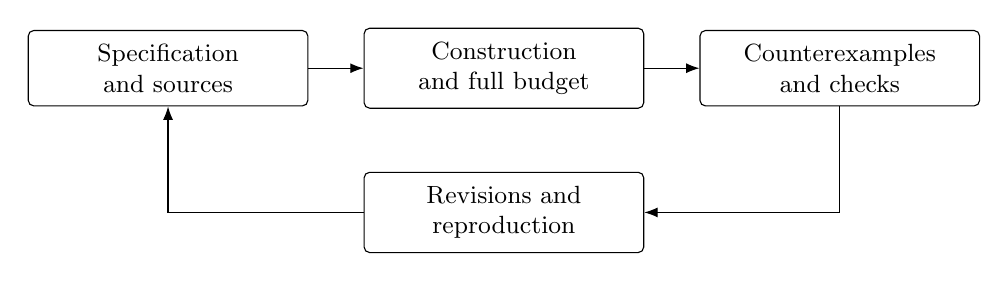
\begin{tikzpicture}[>=Latex,node distance=8mm and 7mm,
 box/.style={draw,rounded corners=2pt,align=center,inner sep=5pt,
 text width=32mm,font=\small}]
\node[box] (s) {Specification\\and sources};
\node[box,right=of s] (p) {Construction\\and full budget};
\node[box,right=of p] (v) {Counterexamples\\and checks};
\node[box,below=of p] (r) {Revisions and\\reproduction};
\draw[->] (s)--(p); \draw[->] (p)--(v);
\draw[->] (v.south)|-(r.east); \draw[->] (r.west)-|(s.south);
\end{tikzpicture}
\caption{A proposed research loop; failed checks are retained as data.}
\end{figure}

\subsubsection{The circuit argument as a stress test}
Section~\ref{sec:main-proof} supplies concrete failure modes that a system
attempting it should be tested against.
\begin{enumerate}[label=(\roman*)]
\item \emph{Length confusion}: keep $n$, $N=dn$, $q(n)$, $2^N$, $s_n$, and
 $U_n$ distinct.
\item \emph{Oracle leakage}: $W\in\ENP$ may use an NP oracle; the fast
 decider for $H$ may not.
\item \emph{Implicit-to-explicit expansion}: writing out $\Phi_n$ inside the
 fast simulation destroys the time bound.
\item \emph{Universal verification}: ``no violated clause'' is an
 unsatisfiability question, decided by the solver, not by an assumed short
 certificate.
\item \emph{Gate accounting}: three copies of $C$, the decoder, signs, and
 the density budget of the encoding.
\item \emph{Quantifier inflation}: the hierarchy contradiction gives
 infinitely many hard lengths, not almost all.
\end{enumerate}
A fluent sketch can fail any one of these while keeping its narrative.

\subsubsection{Acceptance}
\begin{proposition}[Conditional soundness of acceptance]
Assume the semantic correspondence is valid, the logic is sound, and the
correctness and resource certificates have been checked in it. Then an
accepted candidate solves its specified problem within its stated bound.
\end{proposition}
\begin{proof}
The correspondence identifies inputs and outputs, soundness and the
correctness certificate give the output relation, and the resource
certificate gives the bound in the declared model.
\end{proof}
This states the required guarantee; it does not predict that a system will
discover anything.

\subsubsection{Feasibility constraints belong to the proof}
For fixed constants $a,c>0$, consider the exponent
$E(n,b)=an/b+cb\log n$ with $n>1$ and real $b>0$. Unconstrained minimisation gives
$b\asymp\sqrt{n/\log n}$ and $E=O(\sqrt{n\log n})$. If the construction is
valid only for $b\le\log n$, the first term alone is at least $an/\log n$ on
the feasible range. An optimiser needs the validity constraints with the
objective; here they include decoder size, clause density, precision loss,
and the slow variation of $g_\beta$. Minimising a cost expression is not an
existence proof for the object it describes.

\subsection{Evaluation and reproducibility}\label{sec:evaluation}
The architecture has not been implemented here. A useful evaluation would
mix known theorems, new variants, deliberately false lemmas, and open
targets, record training overlap, and compare against equal-budget baselines
with cost verification, counterexample search, or formal checking removed.

\begin{table}[htbp]
\caption{Quantities to report separately.}
\small
\begin{tabularx}{\textwidth}{@{}lY@{}}
\toprule
Quantity & Meaning\\
\midrule
Validated-result rate & outputs passing semantic review and proof checks\\
False acceptance & known-invalid claims accepted as complete\\
Detection cost & time and tool use until an inserted error is found\\
Cost fidelity & missing factors, input overhead, hidden parameters\\
Reproduction & agreement of reruns at pinned versions\\
Human review & expert effort on statement fidelity\\
\bottomrule
\end{tabularx}
\end{table}

\begin{proposition}[What zero observed errors supports]\label{prop:zero-errors}
Let $M\ge1$ and $\alpha\in(0,1)$, and let $M$ cases give independent
Bernoulli error indicators with common probability $\pi$. If no error is
observed, $\pi_U=1-\alpha^{1/M}$ is an exact one-sided upper confidence limit
at level $1-\alpha$, and $\pi_U\sim\ln(1/\alpha)/M$ as $M\to\infty$.
\end{proposition}
\begin{proof}
$(1-\pi)^M<\alpha$ exactly when $\pi>\pi_U$; expand
$\exp((\ln\alpha)/M)$ for the asymptotic form.
\end{proof}
Adaptively selected lemmas, correlated runs, and hand-picked benchmarks need
not satisfy these assumptions; then the raw cases and the selection procedure
should be published instead. A release should contain statements, proofs,
machine and input conventions, pinned dependencies, commands and checker
outputs, and a table matching informal and formal claims. Earlier versions
should remain available when a change alters a theorem's scope.

\begin{thebibliography}{99}
\raggedright
\bibitem{Anthropic}
Anthropic, \emph{A $2^{o(n)}$ time algorithm for 3-SAT}, Hexagon record
2610.00577v1, October 27, 2026.
\href{https://hexagonmath.org/2610.00577v1}{Paper record}.

\bibitem{BackursIndyk}
A. Backurs and P. Indyk, \emph{Edit distance cannot be computed in strongly
subquadratic time (unless SETH is false)}, SIAM J. Comput. \textbf{47}
(2018), no.~3, 1087--1097.
\href{https://arxiv.org/abs/1412.0348}{arXiv:1412.0348}.

\bibitem{Bellman}
R. Bellman, \emph{Dynamic programming treatment of the travelling salesman
problem}, J. ACM \textbf{9} (1962), no.~1, 61--63.
\href{https://doi.org/10.1145/321105.321111}{doi:10.1145/321105.321111}.

\bibitem{Chen}
J. Chen, X. Huang, I. A. Kanj, and G. Xia, \emph{Strong computational lower
bounds via parameterized complexity}, J. Comput. System Sci. \textbf{72}
(2006), no.~8, 1346--1367.
\href{https://doi.org/10.1016/j.jcss.2006.04.007}{doi:10.1016/j.jcss.2006.04.007}.

\bibitem{CHR}
L. Chen, S. Hirahara, and H. Ren, \emph{Symmetric exponential time requires
near-maximum circuit size}, Proc. 56th ACM Symposium on Theory of Computing
(STOC), 2024.
\href{https://arxiv.org/abs/2309.12912}{arXiv:2309.12912};
\href{https://eccc.weizmann.ac.il/report/2023/144/}{ECCC TR23-144}.

\bibitem{CRTY}
L. Chen, R. D. Rothblum, R. Tell, and E. Yogev, \emph{On exponential-time
hypotheses, derandomization, and circuit lower bounds}, Proc. 61st IEEE
Symposium on Foundations of Computer Science (FOCS), 2020; full version ECCC
Report TR19-169.
\href{https://eccc.weizmann.ac.il/report/2019/169/}{ECCC TR19-169}.

\bibitem{DHM}
H. Dell, T. Husfeldt, D. Marx, N. Taslaman, and M. Wahl\'en,
\emph{Exponential time complexity of the permanent and the Tutte
polynomial}, ACM Trans. Algorithms \textbf{10} (2014), no.~4, Article 21.
\href{https://doi.org/10.1145/2635812}{doi:10.1145/2635812}.

\bibitem{FGHK}
M. G. Find, A. Golovnev, E. A. Hirsch, and A. S. Kulikov,
\emph{Improving $3n$ circuit complexity lower bounds}, ECCC Report
TR15-166.
\href{https://eccc.weizmann.ac.il/report/2015/166/}{ECCC TR15-166};
section numbers follow the
\href{https://edwardahirsch.github.io/edwardahirsch/papers/386.pdf}{author's
version} dated August 16, 2022. Conference version: \emph{A better-than-$3n$
lower bound for the circuit complexity of an explicit function}, Proc. 57th
IEEE Symposium on Foundations of Computer Science (FOCS), 2016.

\bibitem{HeldKarp}
M. Held and R. M. Karp, \emph{A dynamic programming approach to sequencing
problems}, J. Soc. Indust. Appl. Math. \textbf{10} (1962), no.~1, 196--210.
\href{https://doi.org/10.1137/0110015}{doi:10.1137/0110015}.

\bibitem{Hoeffding}
W. Hoeffding, \emph{Probability inequalities for sums of bounded random
variables}, J. Amer. Statist. Assoc. \textbf{58} (1963), no.~301, 13--30.
\href{https://doi.org/10.1080/01621459.1963.10500830}{doi:10.1080/01621459.1963.10500830}.

\bibitem{IP}
R. Impagliazzo and R. Paturi, \emph{On the complexity of $k$-SAT},
J. Comput. System Sci. \textbf{62} (2001), no.~2, 367--375.
\href{https://doi.org/10.1006/jcss.2000.1727}{doi:10.1006/jcss.2000.1727}.

\bibitem{IPZ}
R. Impagliazzo, R. Paturi, and F. Zane, \emph{Which problems have strongly
exponential complexity?}, J. Comput. System Sci. \textbf{63} (2001), no.~4,
512--530.
\href{https://cseweb.ucsd.edu/~paturi/myPapers/pubs/ImpagliazzoPaturiZane_2001_jcss.pdf}{Author's version}.
\href{https://doi.org/10.1006/jcss.2001.1774}{doi:10.1006/jcss.2001.1774}.

\bibitem{JMV}
H. Jahanjou, E. Miles, and E. Viola, \emph{Local reductions}, ECCC Report
TR13-099, revision 2, November 27, 2013.
\href{https://eccc.weizmann.ac.il/report/2013/099/revision/2/download/}{Fixed revision}.
Conference version in ICALP 2015, 749--760.
\href{https://arxiv.org/abs/1311.3171}{arXiv:1311.3171}.

\bibitem{JVV}
M. R. Jerrum, L. G. Valiant, and V. V. Vazirani, \emph{Random generation of
combinatorial structures from a uniform distribution}, Theoret. Comput. Sci.
\textbf{43} (1986), nos.~2--3, 169--188.
\href{https://doi.org/10.1016/0304-3975(86)90174-X}{doi:10.1016/0304-3975(86)90174-X}.

\bibitem{Kannan}
R. Kannan, \emph{Circuit-size lower bounds and non-reducibility to sparse
sets}, Inform. and Control \textbf{55} (1982), nos.~1--3, 40--56.
\href{https://doi.org/10.1016/S0019-9958(82)90382-5}{doi:10.1016/S0019-9958(82)90382-5}.

\bibitem{LeanReference}
Lean Language Reference, \emph{Axioms},
\href{https://lean-lang.org/doc/reference/latest/Axioms/}{official reference},
accessed October 28, 2026.

\bibitem{LiYang}
J. Li and T. Yang, \emph{$3.1n-o(n)$ circuit lower bounds for explicit
functions}, Proc. 54th ACM Symposium on Theory of Computing (STOC), 2022.
\href{https://eccc.weizmann.ac.il/report/2021/023/}{ECCC TR21-023}.

\bibitem{LiZ}
Z. Li, \emph{Symmetric exponential time requires near-maximum circuit size:
simplified, truly uniform}, Proc. 56th ACM Symposium on Theory of Computing
(STOC), 2024.
\href{https://arxiv.org/abs/2310.17762v2}{arXiv:2310.17762v2};
\href{https://eccc.weizmann.ac.il/report/2023/156/}{ECCC TR23-156}.

\bibitem{LiptonTarjan}
R. J. Lipton and R. E. Tarjan, \emph{Applications of a planar separator
theorem}, SIAM J. Comput. \textbf{9} (1980), no.~3, 615--627.
\href{https://doi.org/10.1137/0209046}{doi:10.1137/0209046}.

\bibitem{LMS}
D. Lokshtanov, D. Marx, and S. Saurabh, \emph{Lower bounds based on the
Exponential Time Hypothesis}, Bull. EATCS \textbf{105} (2011), 41--72.
\href{https://sites.cs.ucsb.edu/~daniello/papers/surveyETH.pdf}{Author's version}.

\bibitem{MVW}
P. B. Miltersen, N. V. Vinodchandran, and O. Watanabe,
\emph{Super-polynomial versus half-exponential circuit size in the
exponential hierarchy}, COCOON 1999, Lecture Notes in Comput. Sci.
\textbf{1627}, 210--220.
\href{https://doi.org/10.1007/3-540-48686-0_21}{doi:10.1007/3-540-48686-0\_21}.

\bibitem{OpenAIPaper}
OpenAI, \emph{The Exponential Time Hypothesis Is False}, manuscript dated
October 17, 2026, revised October 25, 2026, 67 pp.
\href{https://github.com/openai/math/blob/7ef5c0cc5ca4b0e072b7a050fca09ab24bc6fa3a/preprints/The-Exponential-Time-Hypothesis-is-False-October-25-2026/paper.pdf}{Pinned manuscript}.

\bibitem{OpenAIAnnouncement}
OpenAI, \emph{Working with academic communities to build scientific
understanding}, October 26, 2026.
\href{https://openai.com/index/building-scientific-understanding-with-academic-communities/}{Official announcement},
accessed October 28, 2026.

\bibitem{OpenAIScope}
OpenAI, \emph{The Exponential Time Hypothesis Is False: scope of the Lean
formalization}, \path{lean/docs/378.md}, commit in Appendix~\ref{app:provenance}.
\href{https://github.com/openai/math/blob/7ef5c0cc5ca4b0e072b7a050fca09ab24bc6fa3a/lean/docs/378.md}{Pinned scope document}.

\bibitem{OpenAIComparator}
OpenAI, \emph{SubexponentialSAT comparator statement},
\path{lean/ComparatorChallenges/SubexponentialSAT.lean}, commit in
Appendix~\ref{app:provenance}.
\href{https://github.com/openai/math/blob/7ef5c0cc5ca4b0e072b7a050fca09ab24bc6fa3a/lean/ComparatorChallenges/SubexponentialSAT.lean}{Pinned target}.

\bibitem{Williams}
R. Williams, \emph{Improving exhaustive search implies superpolynomial lower
bounds}, SIAM J. Comput. \textbf{42} (2013), no.~3, 1218--1244.
\href{https://doi.org/10.1137/10080703X}{doi:10.1137/10080703X}.
Theorem and footnote numbers follow the
\href{https://www.cs.cmu.edu/~ryanw/improved-algs-lbs2.pdf}{author's full
version} dated May 4, 2010.

\bibitem{Zak}
S. \v{Z}\'ak, \emph{A Turing machine time hierarchy}, Theoret. Comput. Sci.
\textbf{26} (1983), no.~3, 327--333.
\href{https://doi.org/10.1016/0304-3975(83)90015-4}{doi:10.1016/0304-3975(83)90015-4}.
\end{thebibliography}

\end{document}
%%% Local Variables:
%%% mode: LaTeX
%%% TeX-master: t
%%% End:
